%% The following is a directive for TeXShop to indicate the main file
%%!TEX root = diss.tex

\chapter{Assessment of Formalin-Induced DNA Damage in FFPE Specimens}
\label{ch:AssessmentofFormalin-InducedDNADamageinFFPESpecimens}

The main component of formalin is formaldehyde, which is known to induce DNA damages such as fragmentation and sequence artifacts. Our study design is comprised of 213 patients with FFPE tumour and matched blood specimens that were subjected to evaluation with the OncoPanel. Sequencing data of tumour-normal paired samples were processed and analyzed with a custom variant calling pipeline. With blood specimens serving as non-formalin-fixed controls, we assessed formalin-induced DNA damages by comparing efficiency in amplicon enrichment and sequencing results of FFPE specimens to blood. As DNA derived from blood is the gold standard for germline testing, our assessment would determine whether FFPE DNA is a reliable resource for detection of germline variants.

%%%%%%%%%%%%%%%%%%%%%%%%%%%%%%%%%%%%%%%%%%%%%%%%%%%%%%%%%%%%%%%%%%%%%
\section{Comparison of efficiency in amplicon enrichment and sequencing results between blood and FFPE specimens}
\label{sec:ComparisonofefficiencyinampliconenrichmentandsequencingresultsbetweenbloodandFFPEspecimens}

%%%%%%%%%%%%%%%%%%%%%%%%%%%%%%%%%%%%%%%%%%%%%%%%%%%%%%%%%%%%%%%%%%%%%

Formalin fixation causes DNA fragmentation that would reduce template DNA for PCR amplification, leading to decreased efficiency in amplicon enrichment methods for FFPE DNA. To investigate this effect, we first compared the amplicon yield between blood and FFPE specimens, and a Wilcoxon signed-rank test indicated that amplicon yield in FFPE specimens was significantly lower than blood specimens (\textit{W} = 23613, \textit{Z} = 12.7, \textit{p} = \num{8.3e-62}, \textit{r} = 0.61; \autoref{fig:dna_input_amp_yield}A). However, the amount of DNA input for amplicon enrichment varies across specimens in our study design, and we demonstrated that amplicon yield was weakly correlated with DNA input for both blood and FFPE specimens (Spearman's rank correlation: blood, \textit{r\textsubscript{s}} = 0.29, 95\% CI = 0.16--0.41, \textit{p} = \num{2.1e-5}; FFPE, \textit{r\textsubscript{s}} = 0.25, 95\% CI = 0.12--0.37, \textit{p} = \num{2.5e-4}; \autoref{fig:dna_input_amp_yield}B). To account for the difference in DNA input across specimens, we derived the log2 fold change between DNA input and amplicon yield (log2 (Amplicon Yield/DNA Input)) to measure the efficiency in amplicon enrichment. We compared the log2 fold change in FFPE specimens to blood, and we found a significant decrease in enrichment efficiency in FFPE specimens compared to blood (Wilcoxon signed-rank test, \textit{W} = 24754, \textit{Z} = 12.7, \textit{p} = \num{4.6e-57}, \textit{r} = 0.61; \autoref{fig:dna_input_amp_yield}C). This result implies that production of amplicons is less efficient in FFPE specimens compared to blood, demonstrating the drawback of using FFPE DNA in amplicon-based next-generation sequencing.

To examine whether blood and FFPE specimens produce comparable sequencing results, we compared read alignments between blood and FFPE specimens. Inspection of on-target aligned reads, which are reads that align to target regions used for variant calling, revealed no significant difference in the percentage of on-target aligned reads between blood and FFPE specimens (Wilcoxon signed-rank test, \textit{W} = \num{10178.5}, \textit{Z} = -1.69, \textit{p} = \num{0.091}, \textit{r} = -0.081; \autoref{fig:alignment_pct}). However, there were more outliers with slightly lower percentage of on-target aligned reads ($<$ 75\%) in FFPE specimens compared to blood, and the distribution of percentage of on-target aligned reads was also wider in FFPE specimens (range: FFPE = 32.5--97.4\%, blood = 74.0--95.9\%), suggesting more variability in the rate of on-target alignment in FFPE specimens than blood. Similarly, no significant difference in the percentage of off-target aligned reads, which are reads that map to the human reference genome but not to target regions, was observed between specimen types (Wilcoxon signed-rank test, \textit{W} = \num{11494.5}, \textit{Z} = -0.359, \textit{p} = \num{0.72}, \textit{r} = -0.017; \autoref{fig:alignment_pct}). Although a Wilcoxon signed-rank test indicated that the percentage of unaligned reads was significantly different between blood and FFPE specimens (\textit{W} = \num{19069}, \textit{Z} = 7.82, \textit{p} = \num{2.4e-16}, \textit{r} = 0.38; \autoref{fig:alignment_pct}), there was only a small decrease in the median percentage of unaligned reads in FFPE specimens compared to blood (median: FFPE = 0.8\%, blood = 1.3\%). Moreover, our data showed no significant difference in percentage of contaminant reads between specimen types (\textit{W} = \num{14877}, \textit{Z} = 3.29, \textit{p} = \num{9.2e-4}, \textit{r} = 0.16; \autoref{fig:alignment_pct}), although there was one extreme outlier in FFPE specimens (range: FFPE = 0.028--64\%, blood = 0.082--8.1\%). While there were minor differences in percentage of unaligned reads between sequencing libraries generated from blood and FFPE DNA, blood and FFPE libraries resulted in comparable percentage of on-target aligned reads, thereby providing equivalent amount of aligned reads for variant calling.

Although blood and FFPE specimens demonstrated no significant difference in the percentage of on-target aligned reads, this result does not reflect the coverage depth of target regions in blood and FFPE specimens. To examine whether discrepancy in coverage depth exists between specimen types, we obtained coverage depth of target bases for all sequencing libraries and normalized per base coverage depth to account for difference in library size. We derived the average per base coverage depth for each library and compared this sequencing metric between blood and FFPE specimens. The average per base coverage depth was significantly different between FFPE and blood specimens (Wilcoxon signed-rank test, \textit{W} = \num{20864}, \textit{Z} = 9.76, \textit{p} = \num{2.5e-26}, \textit{r} = 0.47), but there was only a slight decrease in the average per base coverage depth in FFPE specimens compared to blood (median: FFPE = 1194, blood = 1271). We also calculated the percentages of target bases that met coverage thresholds ranging from zero to 1000x to evaluate coverage uniformity of target bases between blood and FFPE specimens. While coverage uniformity was significantly different between blood and FFPE specimens at coverage levels except at the zero and 100x coverage depth cut-off (Wilcoxon signed-rank test, \textit{p} $<$ \num{0.0001}; \autoref{fig:coverage_stats}), we considered these discrepancies to be subtle because the absolute difference in median percentage of target bases only exceeded 5\% at 500x, 900x, and 1000x coverage thresholds (\autoref{tbl:coverage_uniformity}). Nevertheless, there were more outliers with lower percentage of target bases than median values in FFPE specimens at coverage thresholds between 100x to 1000x, implying that poor coverage uniformity is more profound for a subset of FFPE specimens. Together, our findings reveal that FFPE specimens demonstrated lower efficiency in amplicon enrichment and minor discrepancies in coverage depth and uniformity compared to blood specimens, whereas comparable proportion of on-target read alignments could be attained between specimen types.

%%%%%%%%%%%%%%%%%%%%%%%%%%%%%%%%%%%%%%%%%%%%%%%%%%%%%%%%%%%%%%%%%%%%%
%%%%%%%%%%%%%%%%%%%%%%%%%%%%%%%%%%%%%%%%%%%%%%%%%%%%%%%%%%%%%%%%%%%%%

\begin{figure}[H]
	\centering
	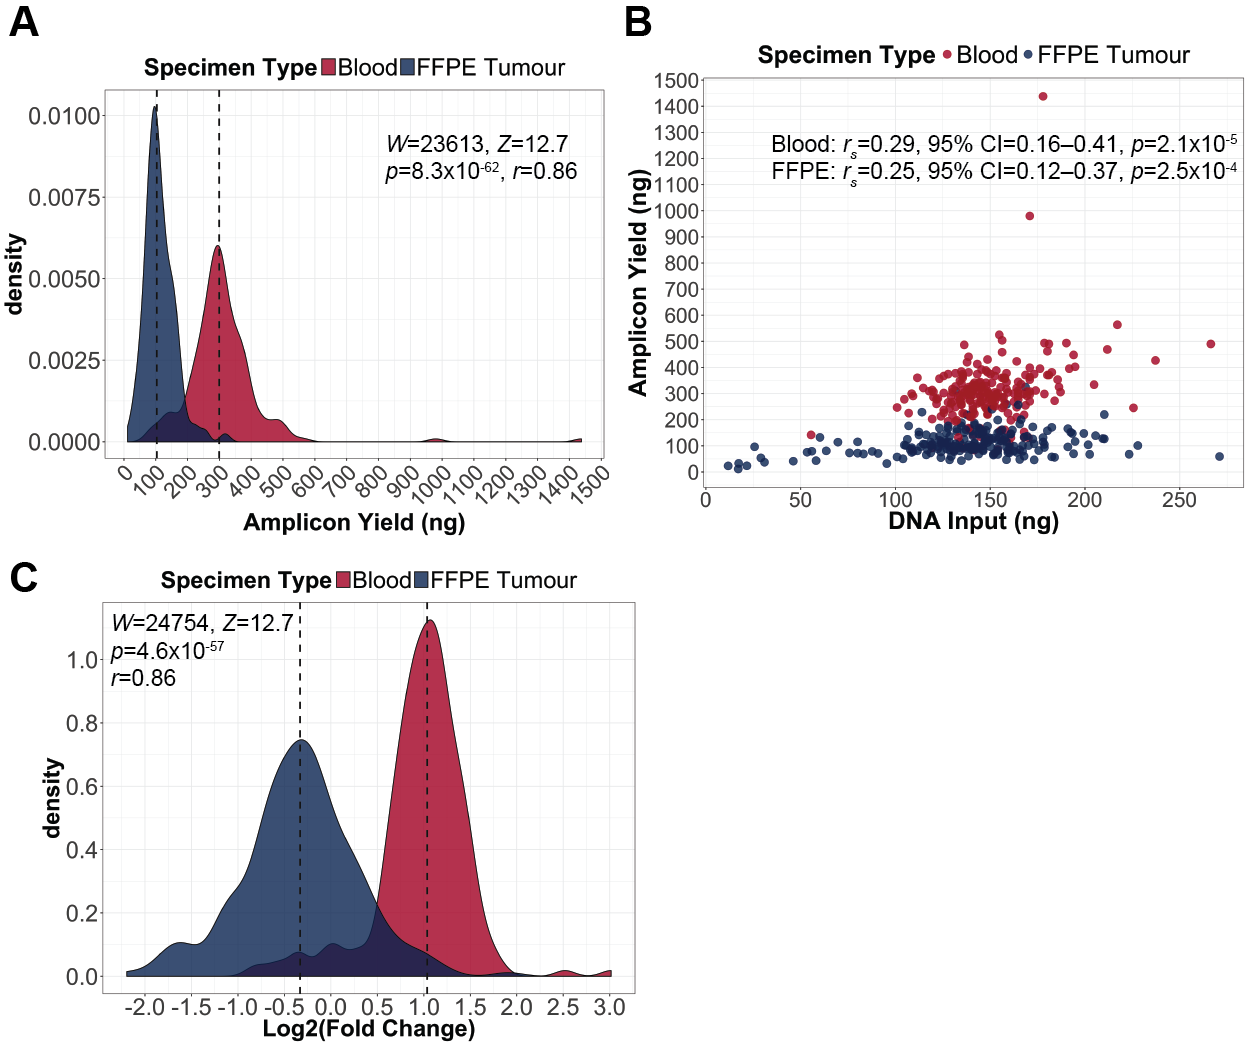
\includegraphics[scale=0.8]{dna_input_amp_yield.png}
	\caption{Comparison of efficiency in amplicon enrichment between blood and FFPE specimens. (A) The distributions of amplicon yield in blood and FFPE specimens (Wilcoxon signed-rank test). Dashed lines indicate median amplicon yield in blood and FFPE specimens, which are 299.3 ng and 103.6 ng, respectively. (B) The correlations between amplicon yield and the amount of DNA input for amplicon enrichment in blood and FFPE specimens (Spearman's rank correlation). (C) The distributions of fold change between DNA input and amplicon yield (log2), which is used to measure efficiency in amplicon enrichment in blood and FFPE specimens (Wilcoxon signed-rank test). Dashed lines indicate median log2 fold change in blood and FFPE specimens, which are 1.04 and -0.332, respectively.}
	\label{fig:dna_input_amp_yield}
\end{figure}

%%%%%%%%%%%%%%%%%%%%%%%%%%%%%%%%%%%%%%%%%%%%%%%%%%%%%%%%%%%%%%%%%%%%%
%%%%%%%%%%%%%%%%%%%%%%%%%%%%%%%%%%%%%%%%%%%%%%%%%%%%%%%%%%%%%%%%%%%%%

\begin{figure}[H]
	\centering
	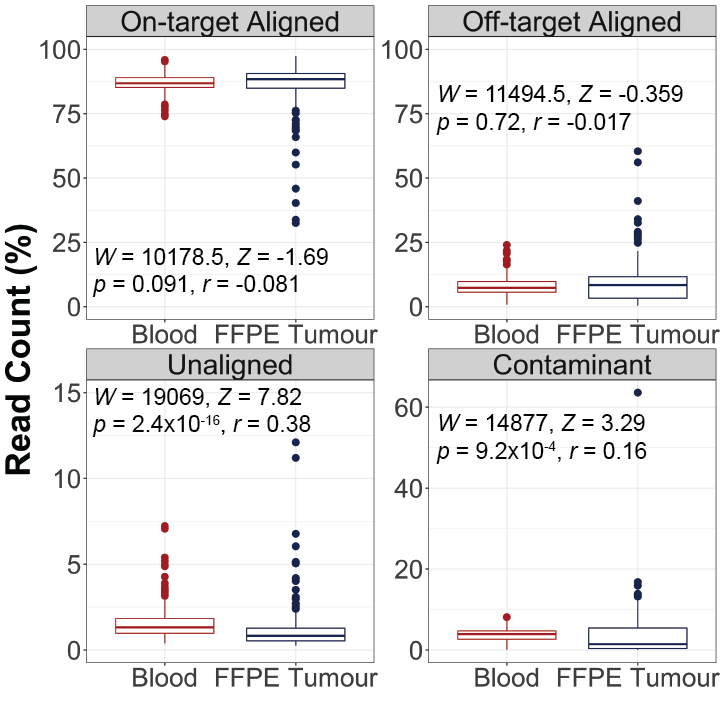
\includegraphics[scale=1]{alignment_pct.png}
	\caption{Assessment of read alignments between blood and FFPE specimens (Wilcoxon signed-rank test). Box plots show the median (horizontal bar within) and interquartile range (IQR) of percentage of reads, with whiskers representing the range of data not exceeding 1.5x the IQR and circles indicating outliers.}
	\label{fig:alignment_pct}
\end{figure}

%%%%%%%%%%%%%%%%%%%%%%%%%%%%%%%%%%%%%%%%%%%%%%%%%%%%%%%%%%%%%%%%%%%%%
%%%%%%%%%%%%%%%%%%%%%%%%%%%%%%%%%%%%%%%%%%%%%%%%%%%%%%%%%%%%%%%%%%%%%

\begin{figure}[H]
	\centering
	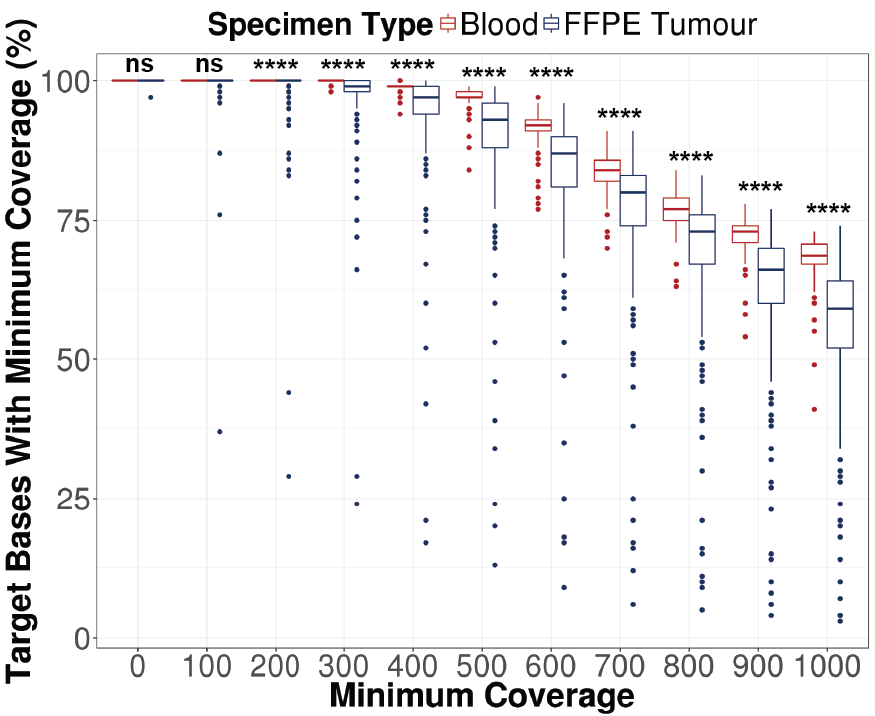
\includegraphics[scale=0.9]{coverage_stats.png}
	\caption{Evaluation of coverage uniformity in blood and FFPE specimens (Wilcoxon signed-rank test, ****\textit{p} $<$ 0.0001, ns = not significant). Per base coverage was normalized to account for difference in library size. Percentage of target bases that met various coverage thresholds was calculated. Box plots show the median (horizontal bar within) and IQR of percentage of target bases that met the respective coverage thresholds, with whiskers representing the range of data not exceeding 1.5x the IQR and circles indicating outliers.}
	\label{fig:coverage_stats}
\end{figure}

%%%%%%%%%%%%%%%%%%%%%%%%%%%%%%%%%%%%%%%%%%%%%%%%%%%%%%%%%%%%%%%%%%%%%
%%%%%%%%%%%%%%%%%%%%%%%%%%%%%%%%%%%%%%%%%%%%%%%%%%%%%%%%%%%%%%%%%%%%%

\begin{table}[H]
\caption{Comparison of coverage uniformity between blood and FFPE specimens using the Wilcoxon signed-rank test.}
\label{tbl:coverage_uniformity}
\centering
      \begin{tabular}{llllllcll}
        \hline
				\multicolumn{1}{l}{ }
				&
				\multicolumn{2}{l}{Blood}
				&&
				\multicolumn{2}{l}{FFPE Tumour}
				&
				\multicolumn{2}{l}{ } \\
				\cline{2-3}\cline{5-6}
        Threshold & Median (\%) & Range (\%) && Median (\%) & Range (\%) & \textit{D}\textsuperscript{$\dagger$} (\%) & \textit{p} ($<$ 0.0001\textsuperscript{*})
				\\
				\hline
				$\geq$ 0x & 100 & 100--100 && 100 & 97.0--100 & 0.0 & 1.0
				\\
				$\geq$ 100x & 100 & 100--100 && 100 & 37.0--100 & 0.0 & \num{2.3e-4}
				\\
				$\geq$ 200x & 100 & 100--100 && 100 & 29.0--100 & 0.0 & \num{2.9e-11}\textsuperscript{*}
				\\
				$\geq$ 300x & 100 & 98.0--100 && 99.0 & 24.0--100 & 1.0 & \num{4.1e-18}\textsuperscript{*}
				\\
				$\geq$ 400x & 99.0 & 94.0--100 && 97.0 & 17.0--100 & 2.0 & \num{5.0e-28}\textsuperscript{*}
				\\
				$\geq$ 500x & 97.0 & 84.0--99.0 && 89.5 & 13.0--99.0 & 7.5 & \num{2.1e-38}\textsuperscript{*}
				\\
				$\geq$ 600x & 92.0 & 77.0--97.0 && 87.0 & 9.0--96.0 & 5.0 & \num{1.5e-32}\textsuperscript{*}
				\\
				$\geq$ 700x & 84.0 & 70.0--91.0 && 80.0 & 6.0--91.0 & 4.0 & \num{5.7e-25}\textsuperscript{*}
				\\
				$\geq$ 800x & 77.0 & 63.0-84.0 && 73.0 & 5.0--83.0 & 4.0 &  \num{4.7e-27}\textsuperscript{*}
				\\
				$\geq$ 900x & 73.0 & 54.0--78.0 && 66.0 & 4.0--77.0 & 7.0 &  \num{4.6e-40}\textsuperscript{*}
				\\
				$\geq$ 1000x & 68.5 & 41.0--73.0 && 59.0 & 3.0-74.0 & 9.5 &  \num{3.6e-42}\textsuperscript{*}
				\\
				\hline
      \end{tabular}
			\justify
			{\small \textsuperscript{$\dagger$}Absolute difference between median of blood and FFPE specimens.}
\end{table}

%%%%%%%%%%%%%%%%%%%%%%%%%%%%%%%%%%%%%%%%%%%%%%%%%%%%%%%%%%%%%%%%%%%%%
\section{Reduced coverage depth in FFPE specimens is more pronounced for longer amplicons}
\label{sec:ReducedcoveragedepthinFFPEspecimensismorepronouncedforlongeramplicons}

The OncoPanel consists of 416 amplicons that interrogate coding exons and mutational hotpots of 21 genes, and these amplicons vary in length and GC content. Since we observed discrepancy in sequencing coverage between blood and FFPE specimens, we sought to determine whether this discrepancy is influenced by amplicon length and GC content. We obtained the coverage depth for each amplicon and normalized the coverage depth to account for difference in library size. We found significant differences in coverage depth between blood and FFPE specimens for 331 out of 416 amplicons (Wilcoxon signed-rank test with Benjamini-Hochberg correction, adjusted \textit{p} $<$ 0.0001; \autoref{fig:amp_norm_depth_med_wilcoxon_volcano}). To quantify the amplicon-specific differences in coverage depth, we derived the log2 fold change in the median coverage depth between blood and FFPE specimens \mbox{(log2 (Median Coverage\textsubscript{FFPE}/Median Coverage\textsubscript{Blood}))} for each amplicon. Hence, a negative fold change indicates lower coverage depth of the amplicon in FFPE specimens relative to blood specimens, whereas a positive fold change indicates higher coverage depth of the amplicon in FFPE specimens relative to blood specimens. Our assessment showed that 217 out of the 331 amplicons have negative log2 fold changes, whereas 114 out of the 331 amplicons have positive log2 fold changes (\autoref{fig:amp_norm_depth_med_wilcoxon_volcano}). These results indicate that there are differences in coverage depth between FFPE and blood specimens for a large proportion of amplicons in the panel, with substantially more amplicons exhibiting lower coverage depth in FFPE specimens than blood specimens.

We subsequently examined the impact of amplicon length and GC content on the amplicon-specific differences in coverage depth between specimen types, which we measured as the log2 fold change in median coverage depth between blood and FFPE specimens. We first confirmed that no significant correlation exists between amplicon GC content and length (Pearson's correlation, \textit{r} = 0.045, 95\% CI = -0.051--0.14, \textit{p} = 0.36; \autoref{fig:amp_gc_length}). We then evaluated the correlation between log2 fold change in amplicon coverage depth and amplicon length, and Pearson's correlation demonstrated a strong, negative correlation between the two variables (\textit{r} = -0.79, 95\% CI = -0.82-- -0.75, \textit{p} = \num{1.4e-88}; \autoref{fig:amp_cov_lm_len_gc}A). This result indicates that coverage depth in FFPE specimens tend to be lower relative to blood specimens as amplicon length increases. On the other hand, coverage depth tend to be enriched in FFPE specimens relative to blood for shorter amplicons. We also assessed the correlation between log2 fold change in amplicon coverage depth and amplicon GC content, and Pearson's correlation demonstrated a weak, negative correlation between the two variables (\textit{r} = -0.31, 95\% CI = -0.40-- -0.22, \textit{p} = \num{1.1e-10}; \autoref{fig:amp_cov_lm_len_gc}B). Although the correlation is weak, this finding still implies that coverage depth in FFPE specimens tend to be lower relative to blood specimens as amplicon GC content increases, whereas enriched coverage depth in FFPE specimens with respect to blood was observed for amplicons with lower GC content.

Because amplicon length and GC content demonstrated significant correlations with amplicon-specific differences in coverage depth, we determined which contributing factor has a greater effect. We used a multiple linear regression to predict log2 fold change in amplicon coverage depth based on amplicon length and GC content (\autoref{tbl:multiple_regression}). A significant equation was found (\textit{F}(2, 411) = 471, \textit{p} = \num{4.65e-107}), with an adjusted \textit{R\textsuperscript{2}} of 0.695. Predicted log2 fold change in amplicon coverage depth between blood and FFPE specimens is equal to $$1.66 - \num{7.24e-3}(\textit{Length}) - \num{9.92e-3}(\textit{GC Content}),$$ in which amplicon length is expressed in base pairs (bp) and GC content is expressed as percentage (\%). Both amplicon length and GC content were significant predictors of log2 fold change in amplicon coverage depth. Based on the standardized coefficients, we compared the strength of predictors within the model to identify the predictor with a greater effect on the response variable. Our assessment showed that one standard deviation increase in amplicon length would lead to a 0.775 standard deviation decrease in log2 fold change in amplicon coverage depth, whereas one standard deviation increase in amplicon GC content would lead to a 0.277 standard deviation decrease in log2 fold change in amplicon coverage depth. This result indicates that amplicon length has a stronger association with amplicon-specific differences in coverage depth between specimen types, which we measured as the log2 fold change in amplicon coverage depth between blood and FFPE specimens, than GC content. Collectively, these findings reveal the challenge imposed by fragmentation damages in FFPE DNA, which results in shorter template DNA that would be more difficult for PCR amplification to produce longer amplicons.

%%%%%%%%%%%%%%%%%%%%%%%%%%%%%%%%%%%%%%%%%%%%%%%%%%%%%%%%%%%%%%%%%%%%%
%%%%%%%%%%%%%%%%%%%%%%%%%%%%%%%%%%%%%%%%%%%%%%%%%%%%%%%%%%%%%%%%%%%%%

\begin{figure}[H]
	\centering
	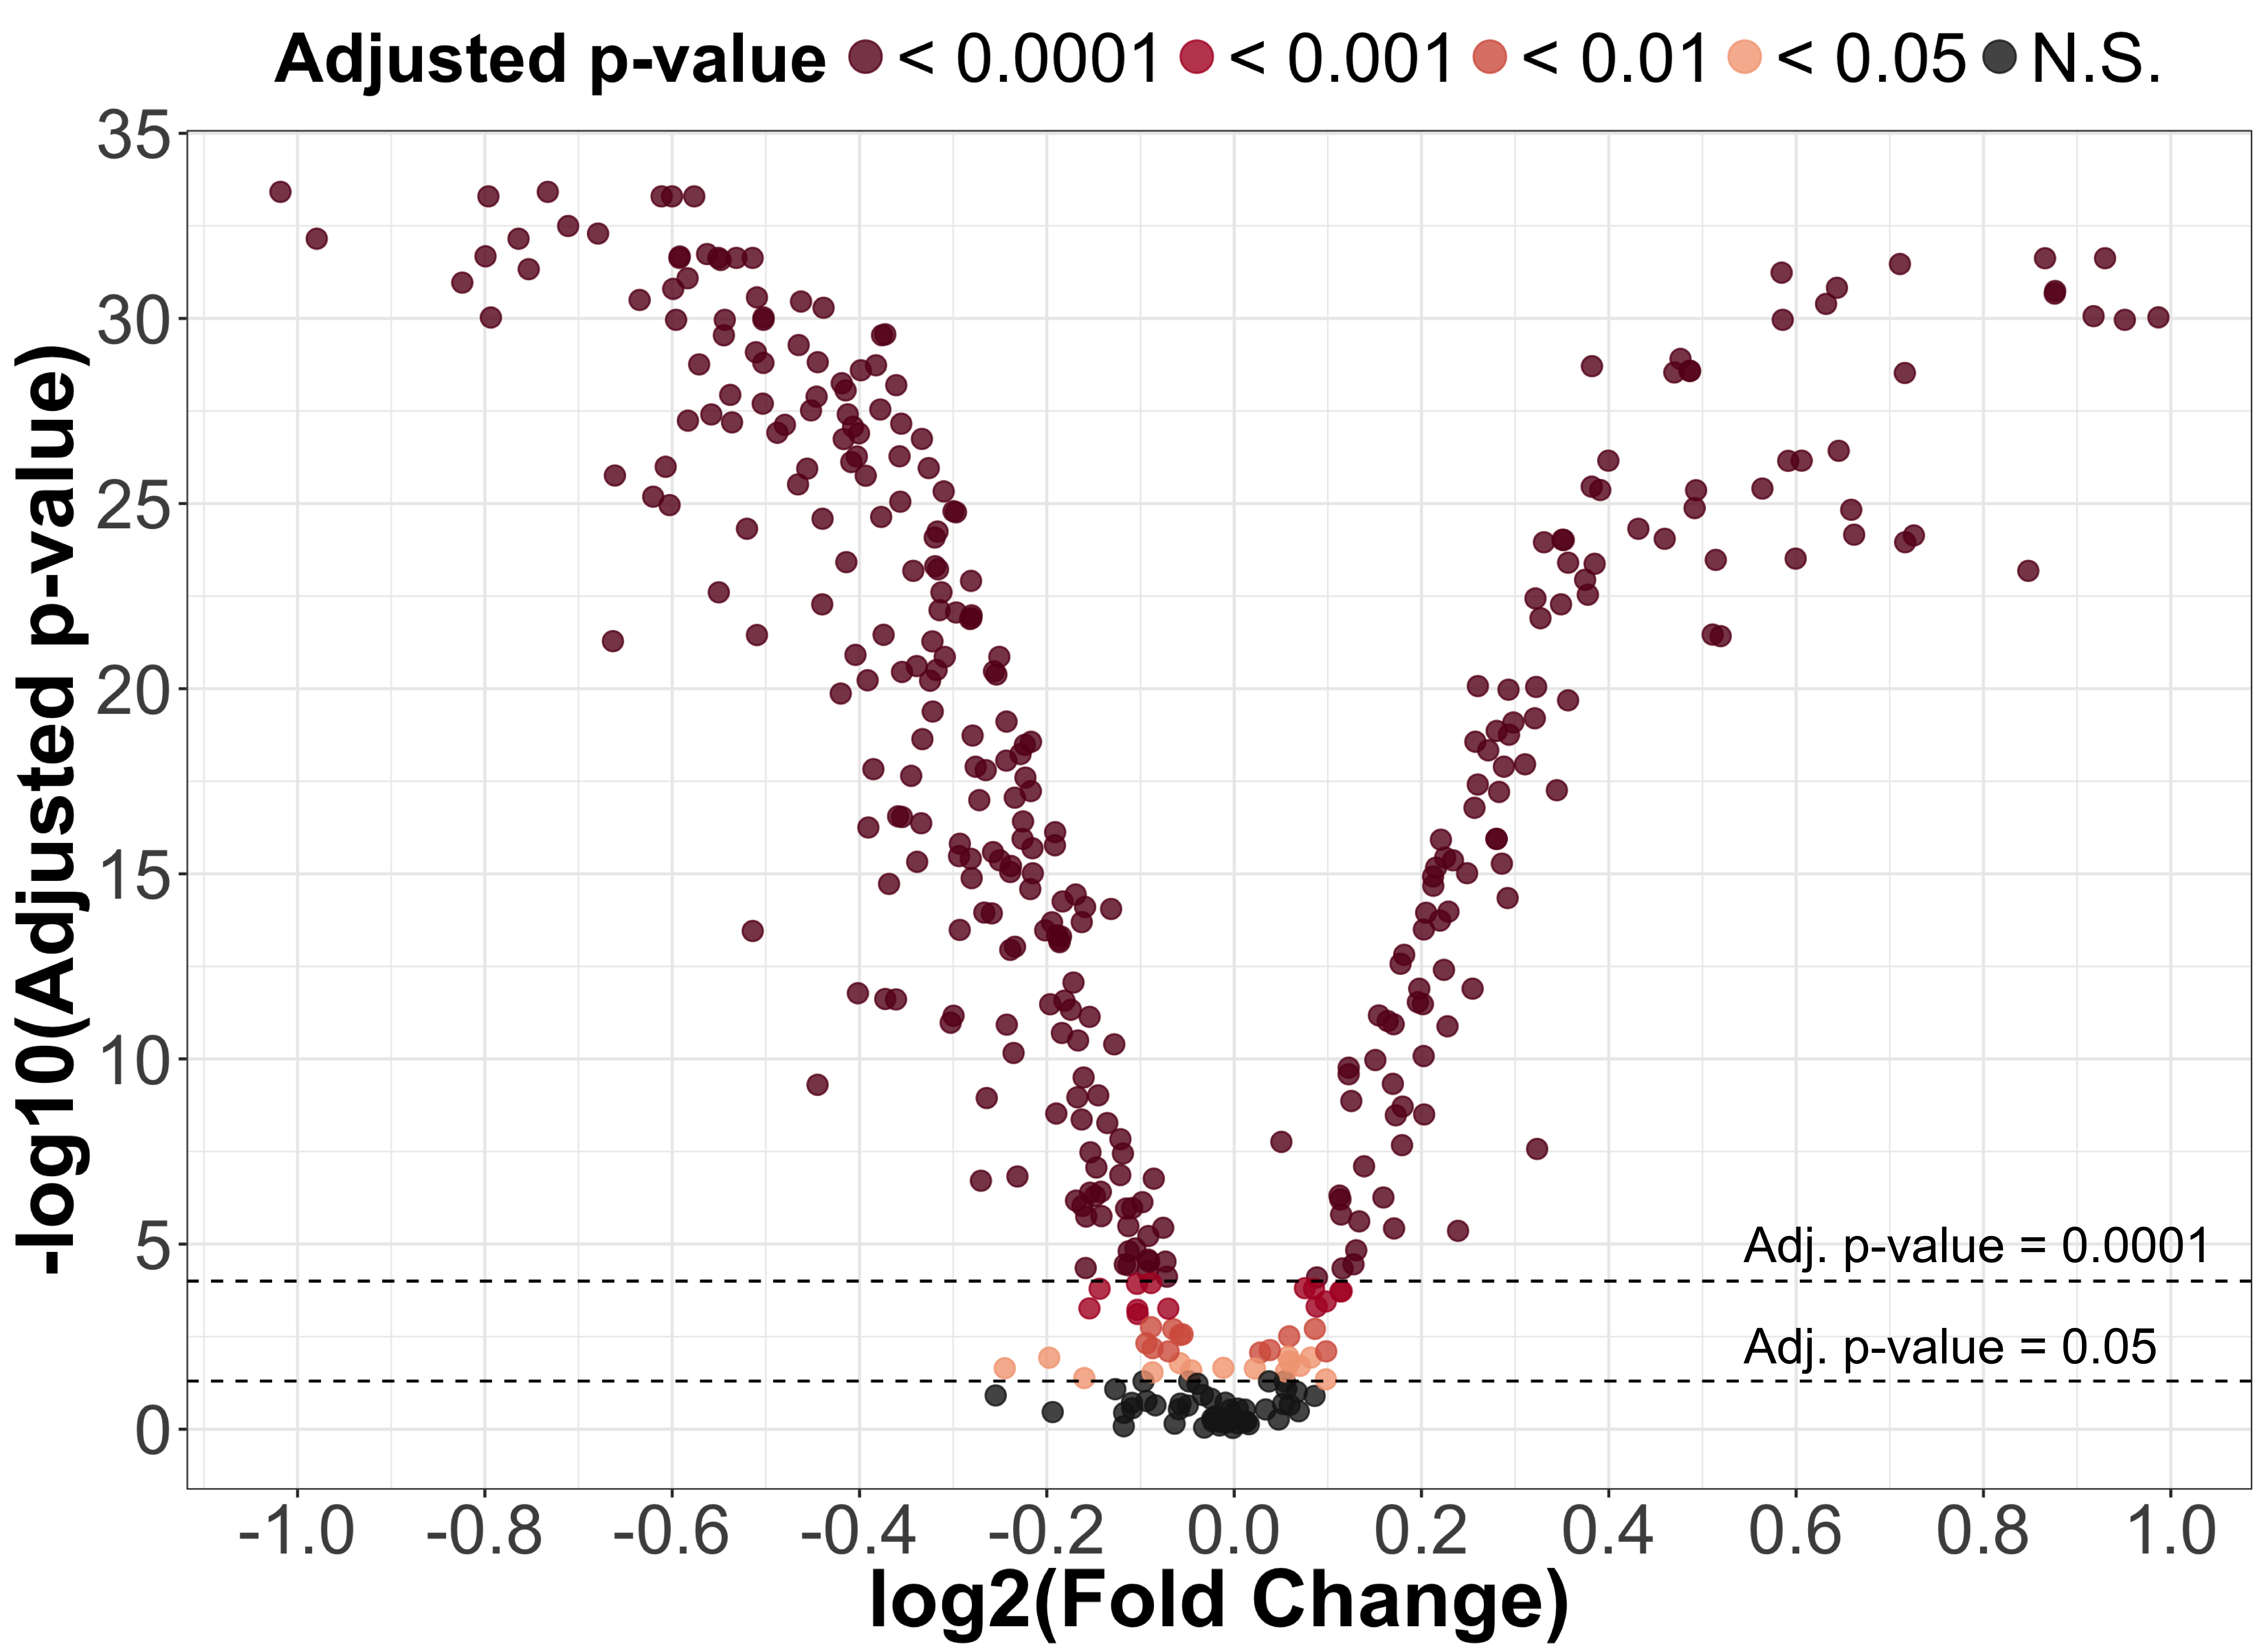
\includegraphics[scale=0.14]{amp_norm_depth_med_wilcoxon_volcano.png}
	\caption{Amplicon-specific differences in coverage depth between blood and FFPE specimens. Difference in amplicon coverage depth between specimen types was determined using the Wilcoxon signed-rank test with Benjamini-Hochberg correction (adjusted \textit{p} $<$ 0.0001). Volcano plot illustrates the -log10 adjusted \textit{p}-value in relation to log2 fold change between median coverage depth in blood and FFPE specimens (\mbox{log2 (Median Coverage\textsubscript{FFPE}/Median Coverage\textsubscript{Blood})}) for amplicons in the panel. Negative log2 fold change indicates lower coverage depth of the amplicon in FFPE specimens relative to blood ($\downarrow \text{Coverage\textsubscript{FFPE}}$), whereas positive log2 fold change indicates higher coverage depth of the amplicon in FFPE specimens relative to blood ($\uparrow\text{Coverage\textsubscript{FFPE}}$). A fold change of 1.5x in either direction, indicated by the dashed lines, was considered to be a substantial change in amplicon coverage depth between blood and FFPE specimens. N = number of amplicons; ns = not significant}
	\label{fig:amp_norm_depth_med_wilcoxon_volcano}
\end{figure}

%%%%%%%%%%%%%%%%%%%%%%%%%%%%%%%%%%%%%%%%%%%%%%%%%%%%%%%%%%%%%%%%%%%%%
%%%%%%%%%%%%%%%%%%%%%%%%%%%%%%%%%%%%%%%%%%%%%%%%%%%%%%%%%%%%%%%%%%%%%

\begin{figure}[H]
	\centering
	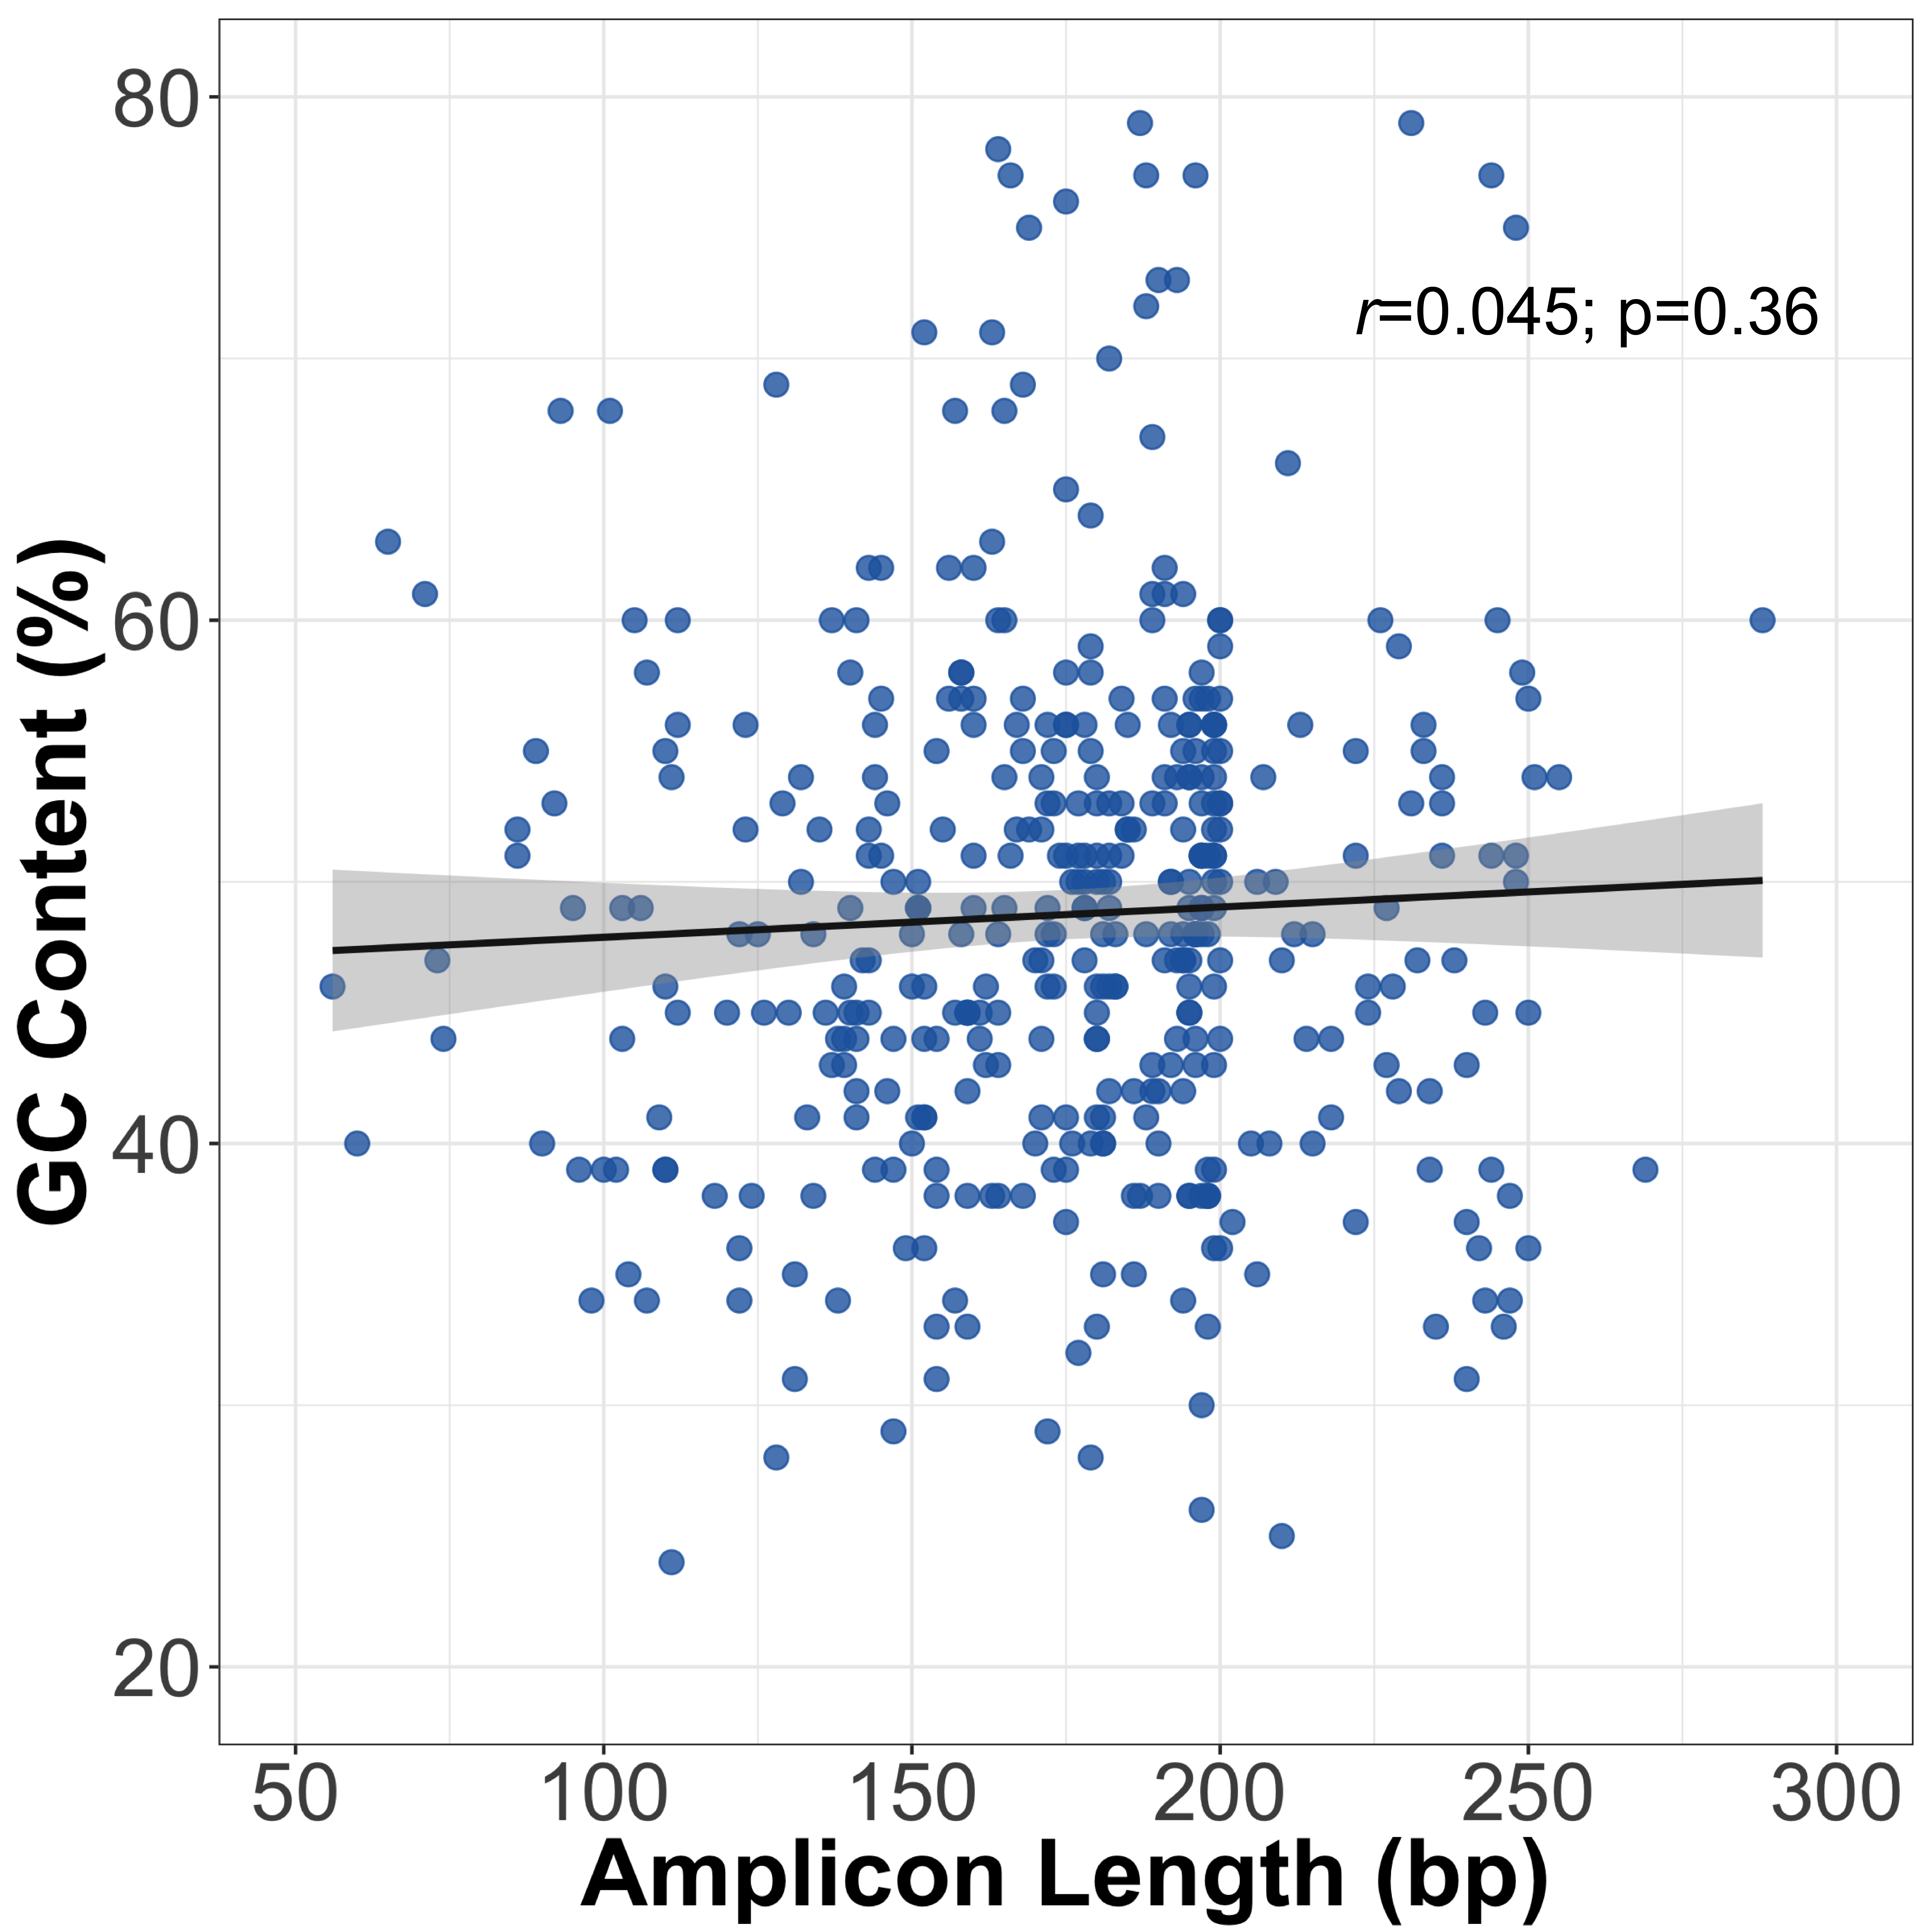
\includegraphics[scale=0.14]{amp_gc_length.png}
	\caption{The relationship between amplicon GC content and amplicon length (Pearson's correlation). Solid line represents the fitted linear relationship between the two variables, and the shaded band indicates pointwise 95\% confidence interval of the fitted linear regression line.}
	\label{fig:amp_gc_length}
\end{figure}

%%%%%%%%%%%%%%%%%%%%%%%%%%%%%%%%%%%%%%%%%%%%%%%%%%%%%%%%%%%%%%%%%%%%%
%%%%%%%%%%%%%%%%%%%%%%%%%%%%%%%%%%%%%%%%%%%%%%%%%%%%%%%%%%%%%%%%%%%%%

\begin{figure}[H]
	\centering
	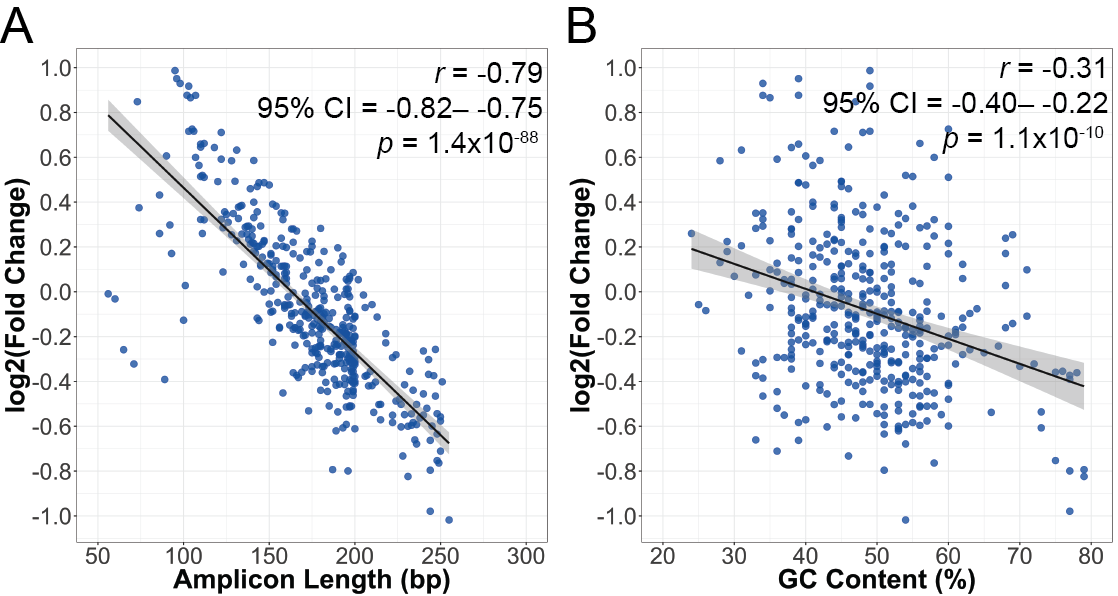
\includegraphics[scale=0.85]{amp_cov_lm_len_gc.png}
	\caption{Scatter plots showing log2 fold change between amplicon coverage depth in blood and FFPE specimens (\mbox{log2 (Median Coverage\textsubscript{FFPE}/Median Coverage\textsubscript{Blood})}) in relation to (A) amplicon length and (B) GC content (Pearson's correlation). Solid line represents the fitted linear relationship between the two variables, and the shaded band indicates pointwise 95\% confidence interval of the fitted linear regression line.}
	\label{fig:amp_cov_lm_len_gc}
\end{figure}

%%%%%%%%%%%%%%%%%%%%%%%%%%%%%%%%%%%%%%%%%%%%%%%%%%%%%%%%%%%%%%%%%%%%%
%%%%%%%%%%%%%%%%%%%%%%%%%%%%%%%%%%%%%%%%%%%%%%%%%%%%%%%%%%%%%%%%%%%%%

\begin{table}[H]
\caption{Multiple linear regression to predict log2 fold change between amplicon coverage depth in blood and FFPE specimens (\mbox{log2 (Median Coverage\textsubscript{FFPE}/Median Coverage\textsubscript{Blood})}) based on amplicon length and GC content.}
\label{tbl:multiple_regression}
\centering
      \begin{tabular}{l|ccccl}
        Variable & Unstandardized Coefficient & Standard Error & Standardized Coefficient & \textit{p}-value
        \\
        \hline
        Length (bp) & \num{-7.24e-3} & \num{2.54e-4} & \num{-7.75e-1} & \num{2.47e-99}
				\\
				GC Content (\%) & \num{-9.92e-3} & \num{9.77e-4} & \num{-2.77e-1} & \num{8.70e-22}
				\\
				\hline
				\\
				 & \multicolumn{4}{r}{Intercept = 1.66, Adjusted R\textsuperscript{2} = 0.695}
				\\
				 & \multicolumn{4}{r}{\textit{F}(2, 411) = 471, \textit{p}-value = \num{4.65e-107}}
				\\
				\hline
      \end{tabular} \\
\end{table}

%%%%%%%%%%%%%%%%%%%%%%%%%%%%%%%%%%%%%%%%%%%%%%%%%%%%%%%%%%%%%%%%%%%%%
\section{Deamination effects lead to increased C$>$T/G$>$A transitions in FFPE specimens}
\label{sec:DeaminationeffectsleadtoincreasedC$>$T/G$>$AtransitionsinFFPEspecimens}

Formalin fixation not only induces DNA fragmentation, but also base modifications that give rise to sequence artifacts. A prominent type of formalin-induced sequence artifact is C$>$T/G$>$A transitions as a result of deamination of cytosine bases. To measure the level of formalin-induced artifacts in FFPE specimens, we quantified the fraction of base changes that were not identified as true SNVs by our variant calling pipeline. We only considered high quality bases (Phred-scaled base quality score $\geq$ 20) and base changes that were $\geq$ 1\% allele frequency to exclude sequencing errors from our analysis. Base changes were categorized into C$>$T/G$>$A and A$>$G/T$>$C, which are nucleotide transitions, as well as C$>$A/G$>$T, A$>$C/T$>$G, C$>$G/G$>$C, and A$>$T/T$>$A, which are nucleotide transversions. We compared the fraction of base changes between specimen types and found significant differences in fraction of C$>$T/G$>$A and A$>$G/T$>$C between blood and FFPE specimens (Wilcoxon signed rank test, \textit{p} $<$ 0.0001; \autoref{fig:deamination_effect_blood_ffpe}A). As blood DNA is not affected by formalin fixation, we evaluated the prevalence of artifactual base changes in FFPE specimens with respect to blood by calculating the fold change between the median fraction of base changes in blood and FFPE specimens (\autoref{tbl:sum_stats_base_changes}). We noted a substantially higher fold change for C$>$T/G$>$A compared to A$>$G/T$>$C: fraction of C$>$T/G$>$A was 23 times higher in FFPE specimens relative to blood, whereas fraction of A$>$G/T$>$C was 3.1 times higher in FFPE specimens relative to blood. This result is consistent with deamination effects that are reportedly predominant in FFPE DNA and considering that base transitions occur at a higher frequency compared to transversions, it is possible that the modest increase in A$>$G/T$>$C transitions was caused by the presence of true SNVs that were not called by our variant calling pipeline.

To assess the relative difference in fraction of base changes in FFPE specimens compared to blood specimens, we calculated the log2 fold change in fraction of base changes between paired blood and FFPE specimens (log2 (Fraction of Base Changes\textsubscript{FFPE}/Fraction of Base Changes\textsubscript{Blood})). We compared the relative difference in fraction of base changes across different types of base changes, and a Kruskal-Wallis test indicated that type of base changes has a significant effect on the relative difference in fraction of base changes (\textit{H} = 428.5, \textit{p} = \num{2.1e-90}; \autoref{fig:deamination_effect_blood_ffpe_fc}). Multiple pairwise comparison of the relative difference in fraction of base changes was performed using a post-hoc Dunn's test with Benjamini-Hochberg correction. Relative difference in fraction of C$>$T/G$>$A was significantly different compared to the five other types of base changes, and this was similar for A$>$G/T$>$C (adjusted \textit{p} $<$ 0.0001; \autoref{tbl:dunntest}). Although both C$>$T/G$>$A and A$>$G/T$>$C were elevated in FFPE specimens compared to the other base transversions, the magnitude of difference was larger for C$>$T/G$>$A than A$>$G/T$>$C (median log2 fold change: C$>$T/G$>$A = 4.2, A$>$G/T$>$C = 1.6), which further confirms that deamination of cytosine bases is the most frequent form of sequence artifacts in FFPE DNA.

Formalin-induced sequence artifacts often occur at low allele frequency; hence, we examined the prevalence of sequence artifacts at different ranges of allele frequency, including 1--10\%, 10-20\%, and 20-30\%. Because variants were not called within the 1--10\% allele frequency range, we did not remove true SNVs detected by our variant calling pipeline to ensure consistency when comparing fraction of base changes across different ranges of allele frequency. Nevertheless, we adhered to the previous criterion of only including base changes with Phred-scaled base quality score $\geq$ 20 in this analysis. For all types of base changes, we noted that the range of allele frequency has a significant effect on fraction of base changes in blood and FFPE specimens (Kruskal-Wallis test, \textit{p} $<$ 0.0001; \autoref{fig:deamination_effect_af_range}), with increased levels of base changes at the 1-10\% allele frequency range compared to 10-20\% and 20-30\%. Because blood DNA represents good quality DNA that is unaffected by formalin fixation, we also compared the fraction of base changes at the 1-10\% allele frequency range in FFPE specimens to blood. Similar to previous analyses, there was a marked increase in C$>$T/G$>$A and a modest increase in A$>$G/T$>$C in FFPE specimens relative to blood within the 1-10\% allele frequency (fold change: C$>$T/G$>$A = 33, A$>$G/T$>$C = 3.1; \autoref{tbl:sum_stats_base_changes_range}). Collectively, our assessment demonstrates that high frequency of C$>$T/G$>$A transitions is present and detectable in FFPE specimens, which indicates that deamination of cytosine is the primary form of formalin-induced sequence artifacts, and these artifactual transitions are more prevalent at low allele frequency.

%%%%%%%%%%%%%%%%%%%%%%%%%%%%%%%%%%%%%%%%%%%%%%%%%%%%%%%%%%%%%%%%%%%%%
%%%%%%%%%%%%%%%%%%%%%%%%%%%%%%%%%%%%%%%%%%%%%%%%%%%%%%%%%%%%%%%%%%%%%

\begin{figure}[H]
	\centering
	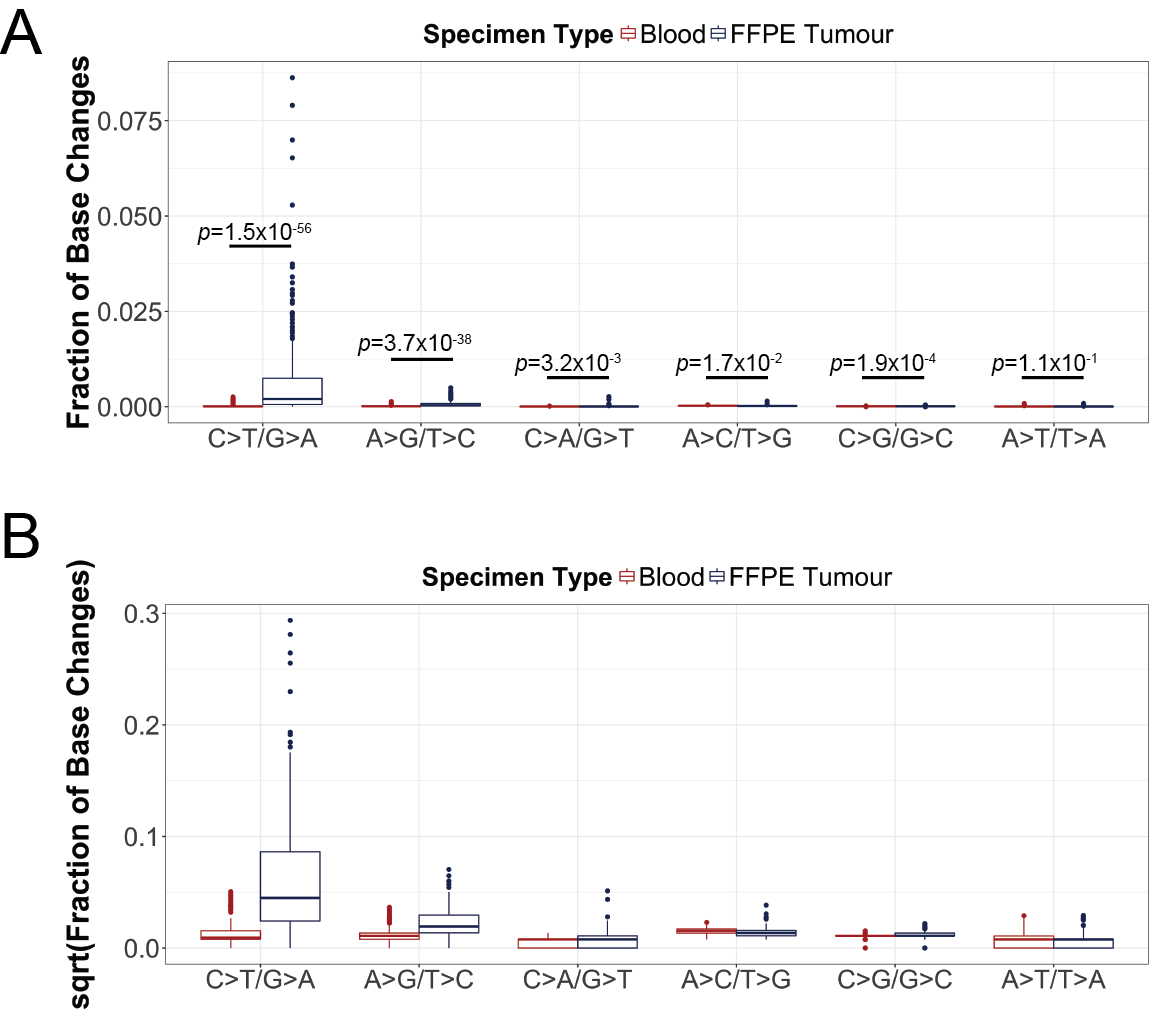
\includegraphics[scale=0.8]{deamination_effect_blood_ffpe.png}
	\caption{Assessment of formalin-induced sequence artifacts in FFPE specimens. (A) Comparison of fraction of base changes in blood and FFPE specimens (Wilcoxon signed-rank test). Box plots show the median (horizontal bar within) and IQR of fraction of base changes for different types of base changes, with whiskers representing the range of data not exceeding 1.5x the IQR and circles indicating outliers. (B) Box plots showing square root-transformed fraction of base changes on the Y-axis.}
	\label{fig:deamination_effect_blood_ffpe}
\end{figure}

%%%%%%%%%%%%%%%%%%%%%%%%%%%%%%%%%%%%%%%%%%%%%%%%%%%%%%%%%%%%%%%%%%%%%
%%%%%%%%%%%%%%%%%%%%%%%%%%%%%%%%%%%%%%%%%%%%%%%%%%%%%%%%%%%%%%%%%%%%%

\begin{table}[H]
\caption{Summary statistics of fraction of base changes in blood and FFPE specimens.}
\label{tbl:sum_stats_base_changes}
\centering
      \begin{tabular}{llllllcl}
        \hline
				\multicolumn{1}{l}{ }
				&
				\multicolumn{2}{l}{Blood}
				&&
				\multicolumn{2}{l}{FFPE Tumour}
				&
				\multicolumn{1}{l}{ } \\
				\cline{2-3}\cline{5-6}
        Type of Base Changes & Median & Range && Median & Range & FC\textsuperscript{$\dagger$}
				\\
				\hline
				C$>$T/G$>$A & \num{8.9e-5} & \num{0}--\num{2.6e-3} && \num{2.0e-3} & \num{0}--\num{8.6e-2} & 23
				\\
				A$>$G/T$>$C & \num{1.2e-4} & \num{0}--\num{1.3e-3} && \num{3.7e-4} & \num{0}--\num{5.0e-3} & 3.1
				\\
				C$>$A/G$>$T & \num{6.0e-5} & \num{0}--\num{1.8e-4} && \num{6.0e-5} & \num{0}--\num{2.6e-3} & 1.0
				\\
				A$>$C/T$>$G & \num{2.4e-4} & \num{5.9e-5}--\num{5.3e-4} && \num{1.8e-4} & \num{5.8e-5}--\num{1.4e-3} & 0.77
				\\
				C$>$G/G$>$C & \num{1.2e-4} & \num{0}--\num{2.4e-4} && \num{1.2e-4} & \num{0}--\num{4.8e-4} & 1.0
				\\
				A$>$T/T$>$A & \num{6.0e-5} & \num{0}--\num{8.4e-4} && \num{5.9e-5} & \num{0}--\num{8.6e-4} & 0.99
				\\
				\hline
      \end{tabular}
			\justify
			{\small \textsuperscript{$\dagger$}Fold change (FC) between the median of blood and FFPE specimens.}
\end{table}

%%%%%%%%%%%%%%%%%%%%%%%%%%%%%%%%%%%%%%%%%%%%%%%%%%%%%%%%%%%%%%%%%%%%%
%%%%%%%%%%%%%%%%%%%%%%%%%%%%%%%%%%%%%%%%%%%%%%%%%%%%%%%%%%%%%%%%%%%%%

\begin{figure}[H]
	\centering
	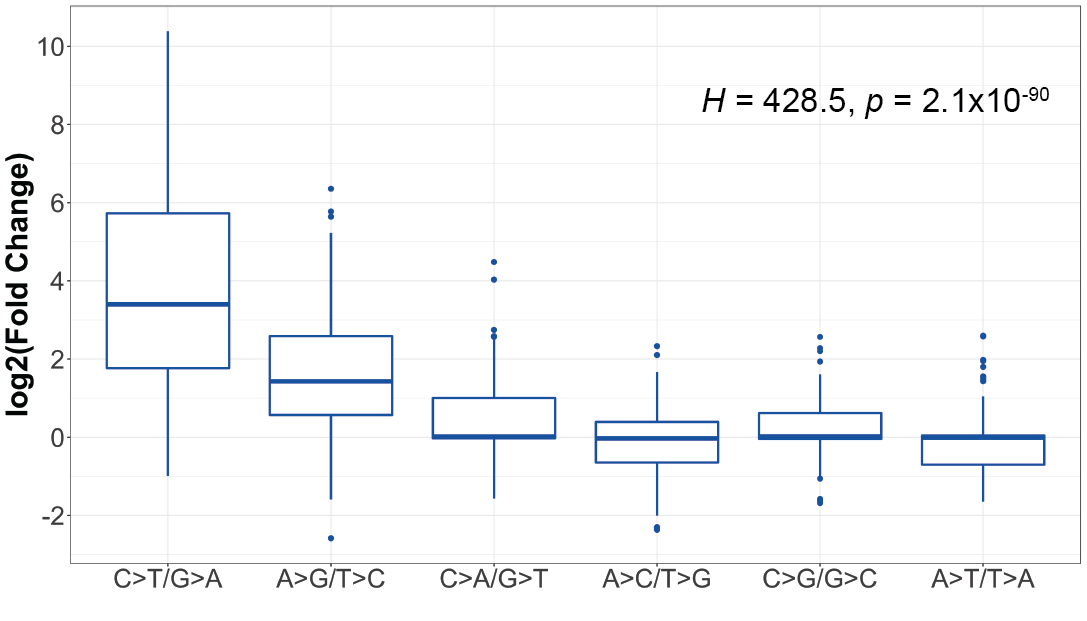
\includegraphics[scale=0.8]{deamination_effect_blood_ffpe_fc.png}
	\caption{Comparison of relative difference in fraction of base changes in FFPE specimens compared to blood (Kruskal-Wallis test). Relative difference was measured as log2 fold change between fraction of base changes in blood and FFPE specimens \mbox{(log2 (Fraction of Base Changes\textsubscript{FFPE}/Fraction of Base Changes\textsubscript{Blood}))}. Box plots show the median (horizontal bar within) and IQR of log2 fold change for different types of base changes, with whiskers representing the range of data not exceeding 1.5x the IQR and circles indicating outliers.}
	\label{fig:deamination_effect_blood_ffpe_fc}
\end{figure}

%%%%%%%%%%%%%%%%%%%%%%%%%%%%%%%%%%%%%%%%%%%%%%%%%%%%%%%%%%%%%%%%%%%%%
%%%%%%%%%%%%%%%%%%%%%%%%%%%%%%%%%%%%%%%%%%%%%%%%%%%%%%%%%%%%%%%%%%%%%

\begin{table}[H]
\caption{Multiple pairwise comparison of log2 fold change in fraction of base changes between blood and FFPE specimens using Dunn's test with Benjamini-Hochberg multiple hypothesis testing correction. Top values represent Dunn's pairwise \textit{z} statistics, whereas bottom values represent adjusted \textit{p}-value. Asterisk(*) indicates significance level of adjusted \textit{p}-value $<$ 0.0001.}
\label{tbl:dunntest}
\centering
      \begin{tabular}{r|l|l|l|l|ll}
        Type of Base Changes & A$>$C/T$>$G & A$>$G/T$>$C & A$>$T/T$>$A & C$>$A/G$>$T & C$>$G/G$>$C
        \\
        \hline
        A$>$G/T$>$C & -11.7 &  &  &  &
        \\
				 & \num{4.15e-31}\mbox{*} &  &  &  &
				\\
				\hline
        A$>$T/T$>$A & -0.399 & 9.57 &  &  &
        \\
				 & \num{3.45e-1} & \num{1.31e-21}\mbox{*} & & &
				\\
				\hline
        C$>$A/G$>$T & -3.46 & 6.39 & -2.73 &  &
        \\
				 & \num{4.00e-4} & \num{1.52e-10}\mbox{*} & \num{3.99e-3} & &
				\\
				\hline
        C$>$G/G$>$C & -3.02 & 8.63 & -2.17 & 0.918 &
				\\
				 & \num{1.73e-3} & \num{6.76e-18}\mbox{*} & \num{1.71e-2} & \num{1.92e-1} &
        \\
				\hline
        C$>$T/G$>$A & -17.1 & -5.60 & -14.3 & -11.1 & -14.1
        \\
				 & \num{7.78e-65}\mbox{*} & \num{1.76e-8}\mbox{*} & \num{5.10e-46}\mbox{*} & \num{1.32e-28}\mbox{*} & \num{6.46e-45}\mbox{*}
				 \\
				\hline
      \end{tabular} \\
\end{table}

%%%%%%%%%%%%%%%%%%%%%%%%%%%%%%%%%%%%%%%%%%%%%%%%%%%%%%%%%%%%%%%%%%%%%
%%%%%%%%%%%%%%%%%%%%%%%%%%%%%%%%%%%%%%%%%%%%%%%%%%%%%%%%%%%%%%%%%%%%%

\begin{figure}[H]
	\centering
	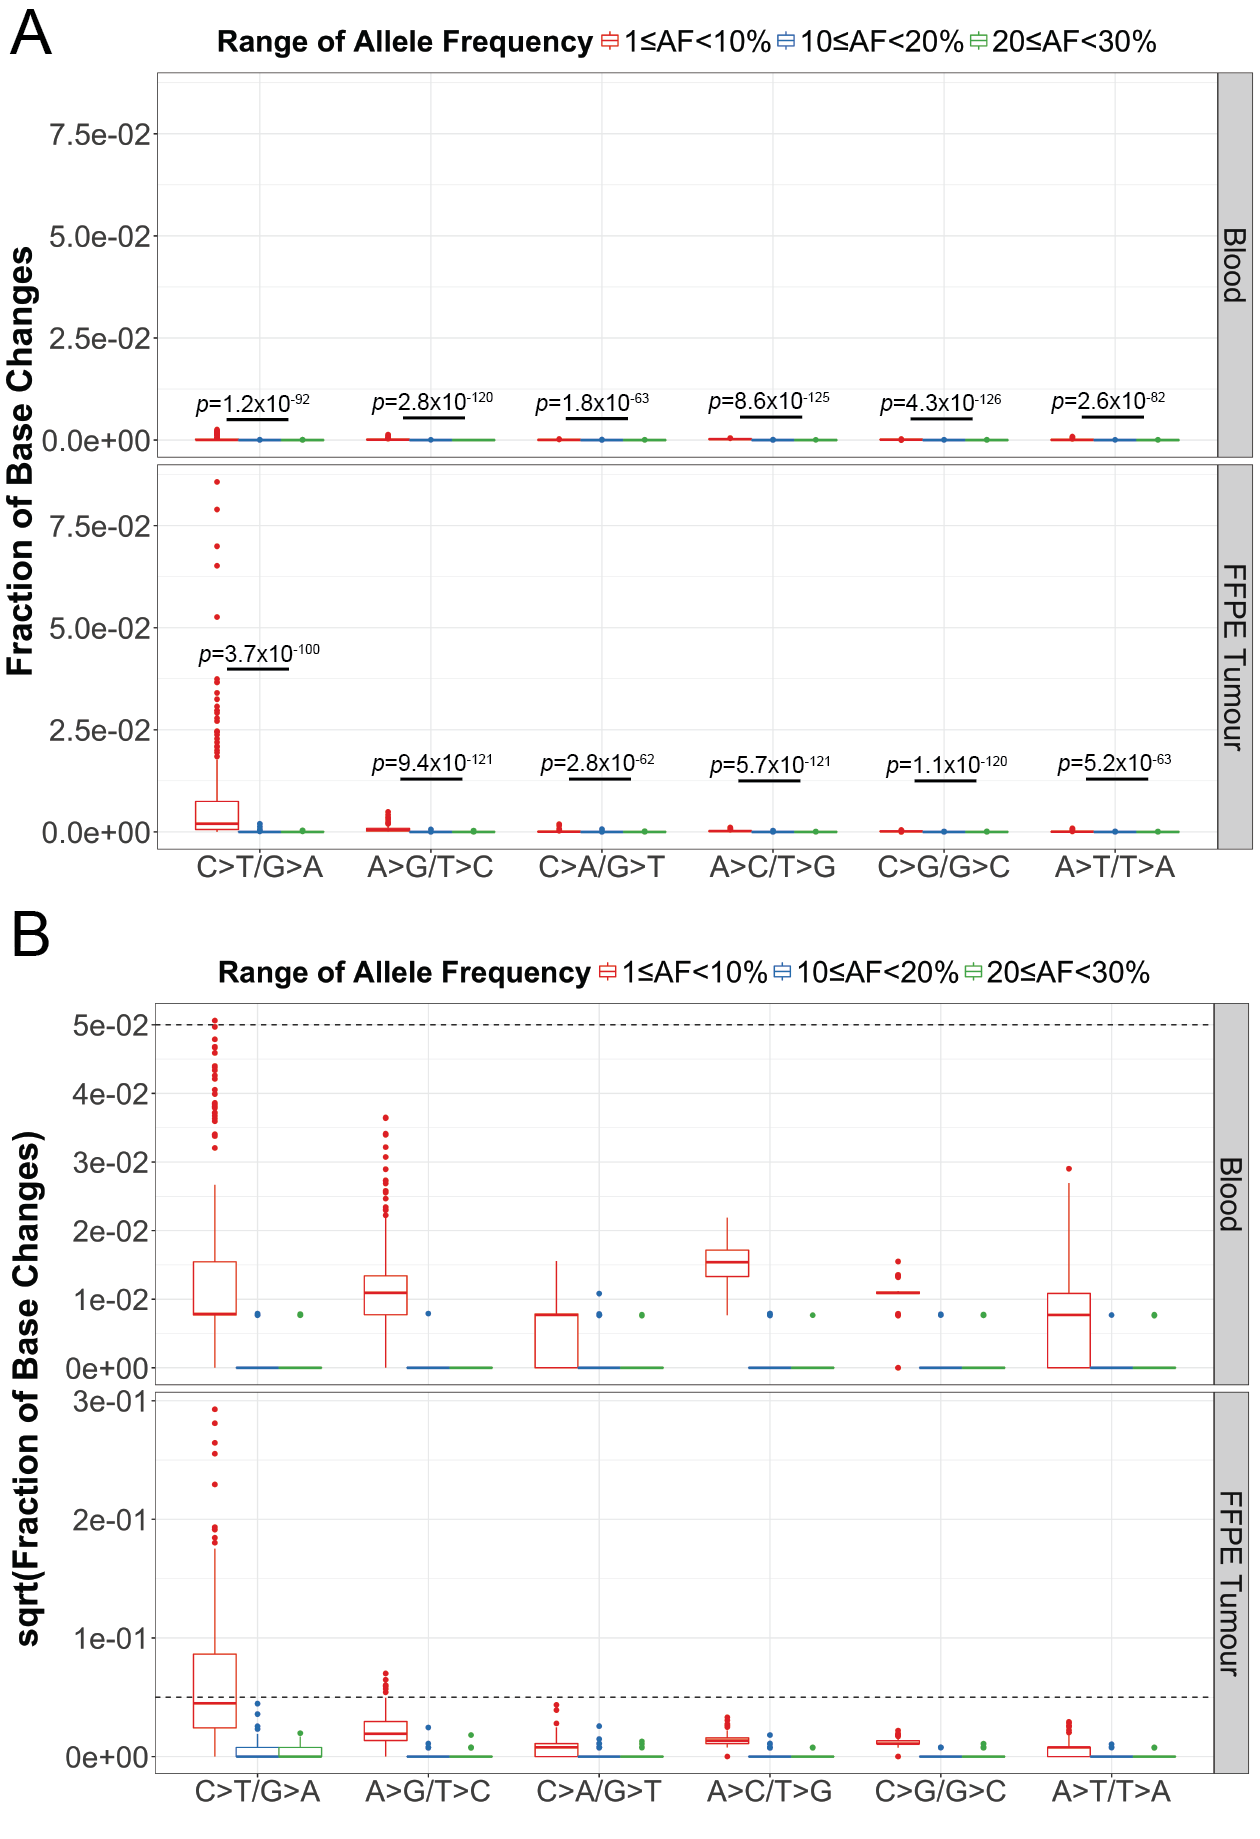
\includegraphics[scale=0.7]{deamination_effect_af_range_2.png}
\end{figure}

%\addtocounter{figure}{-1}
\begin{figure}[H]
	\label{fig:deamination_effect_af_range}
  \caption{Assessment of formalin-induced sequence artifacts in FFPE specimens at different ranges of allele frequency. (A) Comparison of fraction of base changes across different ranges of allele frequency (Kruskal-Wallis test). Box plots show the median (horizontal bar within) and IQR of fraction of base changes for different types of base changes, with whiskers representing the range of data not exceeding 1.5x the IQR and circles indicating outliers. (B) Box plots demonstrating square root-transformed fraction of base changes across different ranges of allele frequency. Dashed lines equal to 0.05 to indicate that the Y-axis scales are different for blood and FFPE tumour plots.}
\end{figure}

%%%%%%%%%%%%%%%%%%%%%%%%%%%%%%%%%%%%%%%%%%%%%%%%%%%%%%%%%%%%%%%%%%%%%
%%%%%%%%%%%%%%%%%%%%%%%%%%%%%%%%%%%%%%%%%%%%%%%%%%%%%%%%%%%%%%%%%%%%%

\newpage
\begin{table}[H]
\caption{Summary statistics of fraction of base changes in blood and FFPE specimens within 1-10\% allele frequency.}
\label{tbl:sum_stats_base_changes_range}
\centering
      \begin{tabular}{llllllcl}
        \hline
				\multicolumn{1}{l}{ }
				&
				\multicolumn{2}{l}{Blood}
				&&
				\multicolumn{2}{l}{FFPE Tumour}
				&
				\multicolumn{1}{l}{ } \\
				\cline{2-3}\cline{5-6}
        Type of Base Changes & Median & Range && Median & Range & \textsuperscript{$\dagger$}FC
				\\
				\hline
				C$>$T/G$>$A & \num{6.2e-5} & \num{0}--\num{2.6e-3} && \num{2.0e-3} & \num{0}--\num{8.6e-2} & 33
				\\
				A$>$G/T$>$C & \num{1.2e-4} & \num{0}--\num{1.3e-3} && \num{3.7e-4} & \num{0}--\num{4.9e-3} & 3.1
				\\
				C$>$A/G$>$T & \num{6.0e-5} & \num{0}--\num{2.4e-4} && \num{6.0e-5} & \num{0}--\num{1.9e-3} & 1.0
				\\
				A$>$C/T$>$G & \num{2.4e-4} & \num{5.9e-5}--\num{4.8e-4} && \num{1.8e-4} & \num{0}--\num{1.1e-3} & 0.77
				\\
				C$>$G/G$>$C & \num{1.2e-4} & \num{0}--\num{2.4e-4} && \num{1.2e-4} & \num{0}--\num{4.8e-4} & 1.0
				\\
				A$>$T/T$>$A & \num{6.0e-5} & \num{0}--\num{8.4e-4} && \num{5.9e-5} & \num{0}--\num{8.6e-4} & 0.99
				\\
				\hline
      \end{tabular}
			\justify
			{\small \textsuperscript{$\dagger$}Fold change (FC) between the median of blood and FFPE specimens.}
\end{table}

%%%%%%%%%%%%%%%%%%%%%%%%%%%%%%%%%%%%%%%%%%%%%%%%%%%%%%%%%%%%%%%%%%%%%
%%%%%%%%%%%%%%%%%%%%%%%%%%%%%%%%%%%%%%%%%%%%%%%%%%%%%%%%%%%%%%%%%%%%%
\section{Increased age of paraffin block results in reduced amplicon yield and elevated level of C$>$T/G$>$A sequence artifacts}
\label{sec:IncreasedageofparaffinblockresultsinpoorerampliconyieldandelevatedeventsofC$>$T/G$>$Asequenceartifacts}

The amount of amplifiable DNA derived from FFPE specimens is dependent on the degree of fragmentation damages. Given two FFPE DNA samples of similar quantity, the sample with more extensive DNA fragmentation would yield reduced amount of PCR amplicons compared to the less fragmented sample. Several studies reported increased fragmentation damages in DNA isolated from older paraffin blocks due to longer exposure to environmental conditions. As the age of paraffin blocks in our study ranges from 18 to 5356 days, we hypothesized that older paraffin blocks would result in more extensively fragmented DNA, leading to reduced efficiency in amplicon enrichment. Inspection of the relationship between amplicon yield and age of paraffin block demonstrated a moderate, negative correlation (Spearman's rank correlation, \textit{r\textsubscript{s}} = -0.42, 95\% CI = -0.52-- -0.30, \textit{p} = \num{1.2e-10}; \autoref{fig:deamination_effect_age_amp_yield}A), suggesting that DNA extraction from older paraffin blocks tend to yield lower amount of amplicons. Because the amount of DNA input for production of amplicons varies across specimens in our study design, a representation of efficiency in amplicon enrichment would be the log2 fold change between DNA input and amplicon yield. Thus, we assessed the correlation between log2 fold change and the storage time of FFPE blocks. Similarly, there was a moderate, negative correlation between log2 fold change and age of paraffin block (Spearman's rank correlation, \textit{r\textsubscript{s}} = -0.42, 95\% CI = -0.53-- -0.30, \textit{p} = \num{1.2e-10}; \autoref{fig:deamination_effect_age_amp_yield}B), implying that production of amplicons is less efficient in FFPE DNA extracted from older paraffin blocks, which is likely caused by more substantial DNA fragmentation.

There are also studies that revealed increased frequency of sequence artifacts in FFPE DNA that are exceedingly fragmented. As DNA fragmentation results in reduced template DNA for PCR amplification, this leads to a higher probability for enrichment of sequence artifacts. Our previous evaluation indicated that older paraffin blocks were associated with lower efficiency in amplicon enrichment, which is possibly due to increased fragmentation damages in the extracted DNA. This leads to our hypothesis that older paraffin blocks would yield elevated levels of sequence artifacts, particularly C$>$T/G$>$A transitions, which are the most prominent type of formalin-induced base modifications. To address our hypothesis, we assessed the relationship between fraction of base changes and age of paraffin blocks for different types of base changes (\autoref{fig:deamination_effect_age}). There was a moderate, positive correlation between fraction of C$>$T/G$>$A transitions and age of paraffin block (Spearman's rank correlation, \textit{r\textsubscript{s}} = 0.54, 95\% CI = 0.43--0.63, \textit{p} = \num{1.0e-17}). We also noted a positive correlation between fraction of A$>$G/T$>$C and age of paraffin block (Spearman's rank correlation, \textit{r\textsubscript{s}} = 0.29, 95\% CI = 0.16--0.40, \textit{p} = \num{2.1e-5}), albeit a weak one. As previously mentioned, it is possible that SNVs with low allele frequencies as a result of clonal heterogeneity were not removed by our variant calling pipeline, resulting in the observed weak correlation for A$>$G/T$>$C. As for transversion base changes (i.e. C$>$A/G$>$T, A$>$C/T$>$G, C$>$G/G$>$C, and A$>$T/T$>$A), no significant correlations with age of paraffin block were observed (Spearman's rank correlation, \textit{p} $<$ \num{0.05}). These findings reveal that increased detection of sequence artifacts, especially the common C$>$T/G$>$A changes in FFPE specimens, is associated with long term storage of FFPE blocks.

We subsequently examined how pre-sequencing variables such as age of paraffin block and efficiency in amplicon enrichment correlate with sequencing metrics, which include average per base coverage (normalized to account for library size), percentage of on-target alignments, and fraction of C$>$T/G$>$A changes (\autoref{tbl:spearman_corr}). This assessment would provide insight on how pre-sequencing variables can affect sequencing results, thereby facilitating sample selection before sequencing. We noted a moderate, negative correlation between average per base coverage and age of paraffin block (Spearman's rank correlation, \textit{r\textsubscript{s}} = -0.47, 95\% CI = -0.57-- -0.36, \textit{p} = \num{4.7e-7}), and a weak, negative correlation between percentage of on-target aligned reads and age of paraffin block (Spearman's rank correlation, \textit{r\textsubscript{s}} = -0.35, 95\% CI = -0.46-- -0.23, \textit{p} = \num{8.2e-3}). Conversely, we observed a moderate, positive correlation between average per base coverage and efficiency in amplicon enrichment (Spearman's rank correlation, \textit{r\textsubscript{s}} = 0.52, 95\% CI = 0.42--0.61, \textit{p} = \num{2.3e-11}), and a weak, positive correlation between percentage of on-target aligned reads and efficiency in amplicon enrichment (Spearman's rank correlation, \textit{r\textsubscript{s}} = 0.35, 95\% CI = 0.22--0.45, \textit{p} = \num{2.9e-5}). Since efficiency in amplicon enrichment is inversely correlated with storage time of FFPE blocks, opposing correlations with sequencing metrics were expected for both pre-sequencing variables. Furthermore, there was also a moderate, negative correlation between fraction of C$>$T/G$>$A and efficiency in amplicon enrichment (Spearman's rank correlation, \textit{r\textsubscript{s}} = -0.55, 95\% CI = -0.64-- -0.45, \textit{p} = \num{2.0e-20}). As reduced efficiency in amplicon enrichment is an indicator for low amount of template DNA, the consequent increase in C$>$T/G$>$A changes is the outcome of stochastic enrichment of sequence artifacts. Together, these results reveal that pre-sequencing variables such as age of paraffin block and efficiency in amplicon enrichment could be predictors of sequencing metrics, in which older FFPE blocks are more likely to yield lower efficiency in amplicon enrichment, leading to poorer sequencing results and increased prevalence of artifactual C$>$T/G$>$A transitions.

%%%%%%%%%%%%%%%%%%%%%%%%%%%%%%%%%%%%%%%%%%%%%%%%%%%%%%%%%%%%%%%%%%%%
%%%%%%%%%%%%%%%%%%%%%%%%%%%%%%%%%%%%%%%%%%%%%%%%%%%%%%%%%%%%%%%%%%%%%

\begin{figure}[H]
	\centering
	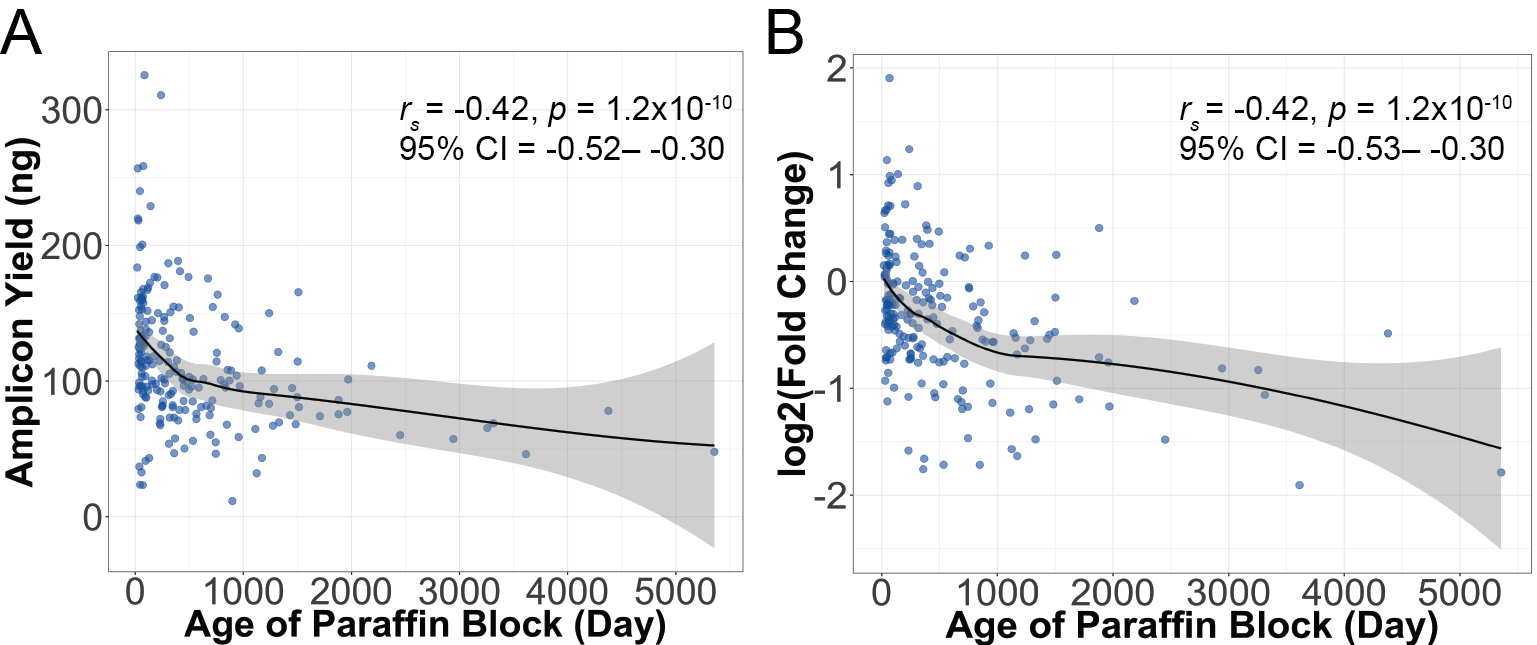
\includegraphics[scale=0.66]{deamination_effect_age_amp_yield.png}
	\caption{Scatter plots showing (A) amplicon yield and (B) efficiency in amplicon enrichment, which is represented by the log2 fold change between the amount of DNA input for producing amplicons and amplicon yield, in relation to age of paraffin blocks (Spearman's rank correlation). Solid lines represent locally weighted smoothing (LOESS) curves, with shaded bands indicating 95\% confidence interval of the LOESS curves.}
	\label{fig:deamination_effect_age_amp_yield}
\end{figure}

%%%%%%%%%%%%%%%%%%%%%%%%%%%%%%%%%%%%%%%%%%%%%%%%%%%%%%%%%%%%%%%%%%%%
%%%%%%%%%%%%%%%%%%%%%%%%%%%%%%%%%%%%%%%%%%%%%%%%%%%%%%%%%%%%%%%%%%%%%

\begin{figure}[H]
	\centering
	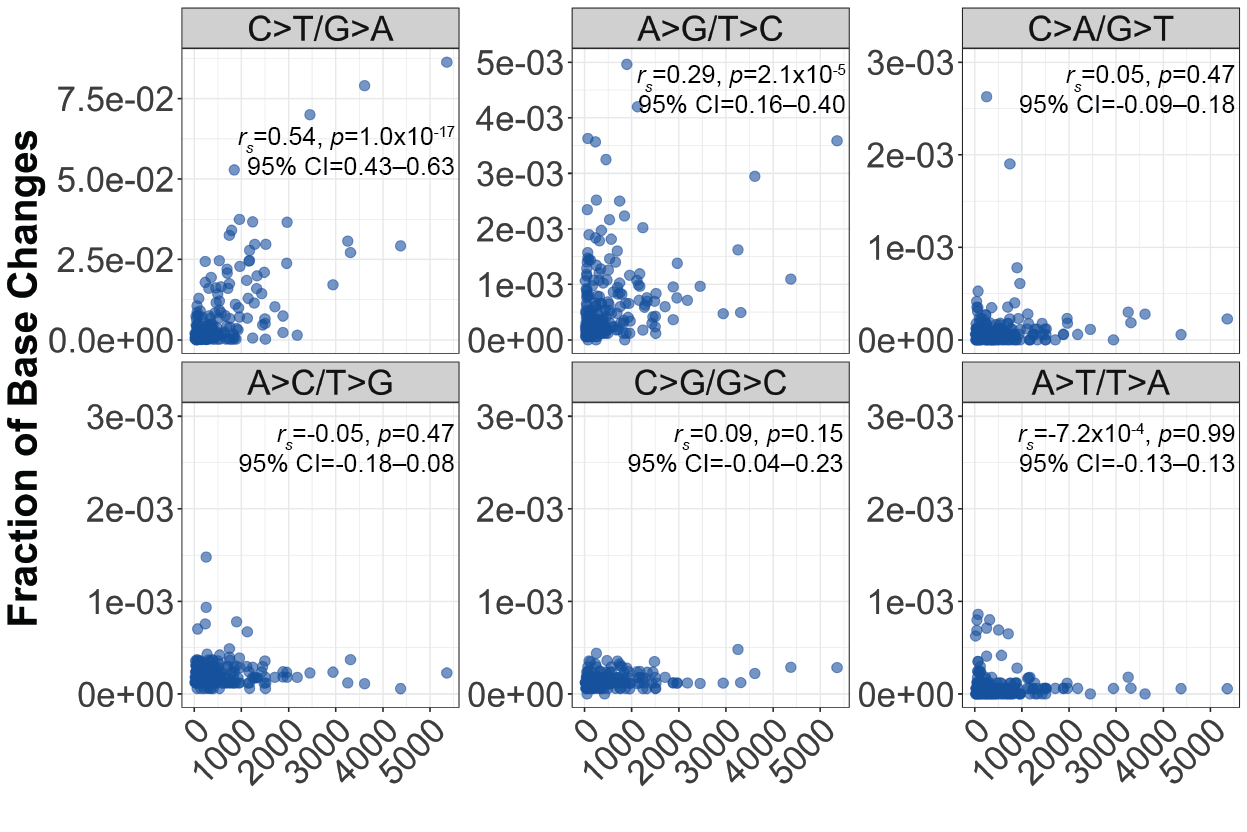
\includegraphics[scale=0.8]{deamination_effect_age.png}
	\caption{The relationship between fraction of base changes and age of paraffin block for different types of base changes (Spearman's rank correlation).}
	\label{fig:deamination_effect_age}
\end{figure}

%%%%%%%%%%%%%%%%%%%%%%%%%%%%%%%%%%%%%%%%%%%%%%%%%%%%%%%%%%%%%%%%%%%%
%%%%%%%%%%%%%%%%%%%%%%%%%%%%%%%%%%%%%%%%%%%%%%%%%%%%%%%%%%%%%%%%%%%%%


\begin{table}[H]
\caption{Spearman's rank correlation between pre-sequencing variables and sequencing metrics. Top values represent Spearman's \textit{rho} and 95\% confidence interval in brackets, whereas bottom values represent \textit{p}-value. Asterisk(*) indicates significance level of \textit{p}-value $<$ 0.05.}
\label{tbl:spearman_corr}
\centering
      \begin{tabular}{l|l|l|l|ll}
        Variable & Enrichment & Age of Paraffin & Fraction of & Average Per Base
        \\
				 & Efficiency\textsuperscript{$\dagger$} & Block (Day) & C$>$T/G$>$A & Normalized Coverage
				\\
        \hline
        Age of Paraffin & -0.42 (-0.53-- -0.30) & & &
				\\
				Block (Day) & \num{9.3e-10}\mbox{*} & & &
        \\
				\hline
				Fraction of & -0.55 (-0.64-- -0.45) & 0.54 (0.43--0.63) & &
				\\
				C$>$T/G$>$A & \num{2.0e-20}\mbox{*} & \num{1.0e-17}\mbox{*} & &
				\\
				\hline
				Average Per Base & 0.52 (0.42--0.61) & -0.47 (-0.57-- -0.36) & -0.80 (-0.84-- -0.75) &
				\\
				Normalized Coverage & \num{2.3e-11}\mbox{*} & \num{4.7e-7}\mbox{*} & \num{7.5e-17}\mbox{*} &
				\\
				\hline
				On-target & 0.34 (0.22--0.45) & -0.35 (-0.46-- -0.23) & -0.57 (-0.65-- -0.47) & 0.73 (0.66--0.79)
				\\
				Aligned Reads (\%) & \num{2.9e-5}\mbox{*} & \num{8.2e-3}\mbox{*} & \num{4.2e-8}\mbox{*} & \num{3.1e-58}\mbox{*}
				\\
				\hline
      \end{tabular} \\
			\justify
			{\small \textsuperscript{$\dagger$}log2 fold change between DNA input for amplicon enrichment and amplicon yield.}
\end{table}

%%%%%%%%%%%%%%%%%%%%%%%%%%%%%%%%%%%%%%%%%%%%%%%%%%%%%%%%%%%%%%%%%%%%%
%%%%%%%%%%%%%%%%%%%%%%%%%%%%%%%%%%%%%%%%%%%%%%%%%%%%%%%%%%%%%%%%%%%%%

\section{Non-reproducible variant calls are detected in sequencing replicates of FFPE specimens}
\label{sec:Non-reproduciblevariantcallsaredetectedinsequencingreplicatesofFFPEspecimens}



%%%%%%%%%%%%%%%%%%%%%%%%%%%%%%%%%%%%%%%%%%%%%%%%%%%%%%%%%%%%%%%%%%%%%
\endinput
%%%%%%%%%%%%%%%%%%%%%%%%%%%%%%%%%%%%%%%%%%%%%%%%%%%%%%%%%%%%%%%%%%%%%

%%%%%%%%%%%%%%%%%%%%%%%%%%%%%%%%%%%%%%%%%%%%%%%%%%%%%%%%%%%%%%%%%%%%%

\begin{table}[H]
\caption{Assessment of amplicon enrichment results in blood and FFPE specimens. \textit{p} value indicates significance level for Wilcoxon signed-rank test.}
\label{tbl:amplicon_generation}
			\begin{tabular}{lllllll}
				\hline
			 \multicolumn{1}{l}{ }
			 &
			 \multicolumn{2}{l}{Blood}
			 &&
			 \multicolumn{2}{l}{FFPE Tumour}
			 &
			 \multicolumn{1}{l}{ } \\
			 \cline{2-3}\cline{5-6}
			 Parameter & Median & Range && Median & Range & \textit{p} ($<$ 0.05\textsuperscript{*})
			 \\
			 \hline
			 Amplicon Yield (ng) & 299.3 & 84.0--1438.0 && 103.6 & 11.6--325.5 & \num{8.3e-62}\textsuperscript{*}
			 \\
			 DNA Input (ng) & 147.8 & 55.5--266.4 && 140.9 & 11.8--271.0 & \num{3.2e-4}\textsuperscript{*}
			 \\
			 log2(\( \frac{\text{Amplicon Yield}}{\text{DNA Input}} \)) & 1.04 & -0.845--3.01 && -0.332 & -2.20--1.90 & \num{4.6e-57}\textsuperscript{*}
			 \\
			 \hline
			\end{tabular} \\
\end{table}

%%%%%%%%%%%%%%%%%%%%%%%%%%%%%%%%%%%%%%%%%%%%%%%%%%%%%%%%%%%%%%%%%%%%%
%%%%%%%%%%%%%%%%%%%%%%%%%%%%%%%%%%%%%%%%%%%%%%%%%%%%%%%%%%%%%%%%%%%%%

\begin{table}[H]
\caption{Comparison of read alignments between blood and FFPE specimens. \textit{p} value indicates significance level for Wilcoxon signed-rank test.}
\label{tbl:alignment}
      \begin{tabular}{lllllll}
        \hline
				\multicolumn{1}{l}{ }
				&
				\multicolumn{2}{l}{Blood}
				&&
				\multicolumn{2}{l}{FFPE Tumour}
				&
				\multicolumn{1}{l}{ } \\
				\cline{2-3}\cline{5-6}
        Parameter & Median & Range && Median & Range & \textit{p} ($<$ 0.05\textsuperscript{*})
				\\
				\hline
				On-target Aligned Reads (\%) & 86.8 & 74.0--95.9 && 88.4 & 32.5--97.4 & \num{0.091}
				\\
				Off-target Aligned Reads (\%) & 7.3 & 0.8--24.0 && 8.4 & 0.4--60.4 & \num{0.72}
				\\
				Unaligned Reads (\%) & 1.3 & 0.4--7.2 && 0.8 & 0.3--12.1 & \num{2.4e-16}\textsuperscript{*}
				\\
				Contaminant (\%) & 3.9 & 0.1--8.1 && 1.4 & 0.03--63.6 &
				\num{9.2e-4}\textsuperscript{*}
				\\
				\hline
      \end{tabular} \\
\end{table}

%%%%%%%%%%%%%%%%%%%%%%%%%%%%%%%%%%%%%%%%%%%%%%%%%%%%%%%%%%%%%%%%%%%%%
%%%%%%%%%%%%%%%%%%%%%%%%%%%%%%%%%%%%%%%%%%%%%%%%%%%%%%%%%%%%%%%%%%%%%

\begin{table}[H]
\caption{Comparison of coverage uniformity between blood and FFPE specimens using the Wilcoxon signed-rank test.}
\label{tbl:metrics}
\centering
      \begin{tabular}{llllllllll}
        \hline
				\multicolumn{1}{l}{ }
				&
				\multicolumn{2}{l}{Blood}
				&&
				\multicolumn{2}{l}{FFPE Tumour}
				&
				\multicolumn{4}{l}{ } \\
				\cline{2-3}\cline{5-6}
        Threshold & Median (\%) & Range (\%) && Median (\%) & Range (\%) & \textit{W} & \textit{Z} & \textit{p} ($<$ 0.05\textsuperscript{*}) & \textit{r}
				\\
				\hline
				$\geq$ 0x & 100.0 & 100.0--100.0 && 100.0 & 97.0--100.0 & 1 & 1.00 & 1.0 & 0.068
				\\
				$\geq$ 100x & 100.0 & 100.0--100.0 && 100.0 & 37.0--100.0 & 91 & 3.61 & \num{2.3e-4}\textsuperscript{*} & 0.25
				\\
				$\geq$ 200x & 100.0 & 100.0--100.0 && 100.0 & 29.0--100.0 & 666 & 5.99 & \num{2.9e-11}\textsuperscript{*} & 0.41
				\\
				$\geq$ 300x & 100.0 & 98.0--100.0 && 99.0 & 24.0--100.0 & 7696 & 8.17 & \num{4.1e-18}\textsuperscript{*} & 0.55
				\\
				$\geq$ 400x & 99.0 & 94.0--100.0 && 97.0 & 17.0--100.0 & 13934 & 10.0 & \num{5.0e-28}\textsuperscript{*} & 0.68
				\\
				$\geq$ 500x & 97.0 & 84.0--99.0 && 89.5 & 13.0--99.0 & 19880.5 & 11.3 & \num{2.1e-38}\textsuperscript{*} & 0.77
				\\
				$\geq$ 600x & 92.0 & 77.0--97.0 && 87.0 & 9.0--96.0 & 20762 & 10.6 & \num{1.5e-32}\textsuperscript{*} & 0.72
				\\
				$\geq$ 700x & 84.0 & 70.0--91.0 && 80.0 & 6.0--91.0 & 18458.5 & 9.54 & \num{5.7e-25}\textsuperscript{*} & 0.65
				\\
				$\geq$ 800x & 77.0 & 63.0-84.0 && 73.0 & 5.0--83.0 & 18127 & 9.87 & \num{4.7e-27}\textsuperscript{*} & 0.67
				\\
				$\geq$ 900x & 73.0 & 54.0--78.0 && 66.0 & 4.0--77.0 & 20706 & 11.5 & \num{4.6e-40}\textsuperscript{*} & 0.78
				\\
				$\geq$ 1000x & 68.5 & 41.0--73.0 && 59.0 & 3.0-74.0 & 21054.5 & 11.7 & \num{3.6e-42}\textsuperscript{*} & 0.79
				\\
				\hline
      \end{tabular} \\
\end{table}

%%%%%%%%%%%%%%%%%%%%%%%%%%%%%%%%%%%%%%%%%%%%%%%%%%%%%%%%%%%%%%%%%%%%%
% Orphaned text
%%%%%%%%%%%%%%%%%%%%%%%%%%%%%%%%%%%%%%%%%%%%%%%%%%%%%%%%%%%%%%%%%%%%%

the median coverage depth of amplicons and amplicon length in both blood and FFPE specimens (\autoref{fig:amp_cov_lm_len}A). While we found no significant correlation between median coverage depth and amplicon length in blood specimens (Pearson's correlation, \textit{r} = 0.042, 95\% CI = -0.054--0.14, \textit{p} = 0.39), we observed a negative correlation in FFPE specimens (Pearson's correlation, \textit{r} = -0.28, 95\% CI = -0.37-- -0.19, \textit{p} = \num{7.4e-9}). We evaluated the relationship between the discrepancy in amplicon coverage depth between FFPE and blood specimens, which was calculated as the log2 fold change from the median coverage depth in blood specimens to the median coverage depth in FFPE specimens (log2\( \frac{\text{Median Coverage Depth in FFPE}}{\text{Median Coverage Depth in Blood}} \)), and amplicon length (\autoref{fig:amp_cov_lm_len}B).

To assess the effect of amplicon GC content on coverage depth of amplicons, we explored the correlation between the median coverage depth of amplicons and amplicon GC content in blood and FFPE specimens (\autoref{fig:amp_cov_lm_gc}A). Using Pearson's correlation, we identified weak, negative correlations between median coverage depth and amplicon GC content in both blood and FFPE specimens (blood: \textit{r} = -0.16, 95\% CI = -0.25-- -0.067, \textit{p} = \num{8.7e-4}; FFPE: \textit{r} = -0.29, 95\% CI = -0.38-- -0.20 \textit{p} = \num{1.0e-9}). We next assessed the relationship between the discrepancy in amplicon coverage depth between FFPE and blood specimens (log2\( \frac{\text{Median Coverage Depth in FFPE}}{\text{Median Coverage Depth in Blood}} \)) and amplicon GC content (\autoref{fig:amp_cov_lm_gc}B). In contrast to the strong, negative correlation observed for the log2 fold change in amplicon coverage depth in relation to amplicon length, Pearson's correlation demonstrated a weak, negative correlation between the log2 fold change in amplicon coverage depth and amplicon GC content (\textit{r} = -0.31, 95\% CI = -0.40-- -0.22, \textit{p} = \num{1.1e-10}). While the correlation is weak, this finding still implies that increased amplicon GC content has a significant impact on the decrease in amplicon coverage depth in FFPE specimens relative to blood specimens.

%%%%%%%%%%%%%%%%%%%%%%%%%%%%%%%%%%%%%%%%%%%%%%%%%%%%%%%%%%%%%%%%%%%%%
%%%%%%%%%%%%%%%%%%%%%%%%%%%%%%%%%%%%%%%%%%%%%%%%%%%%%%%%%%%%%%%%%%%%%

\begin{figure}[H]
	\centering
	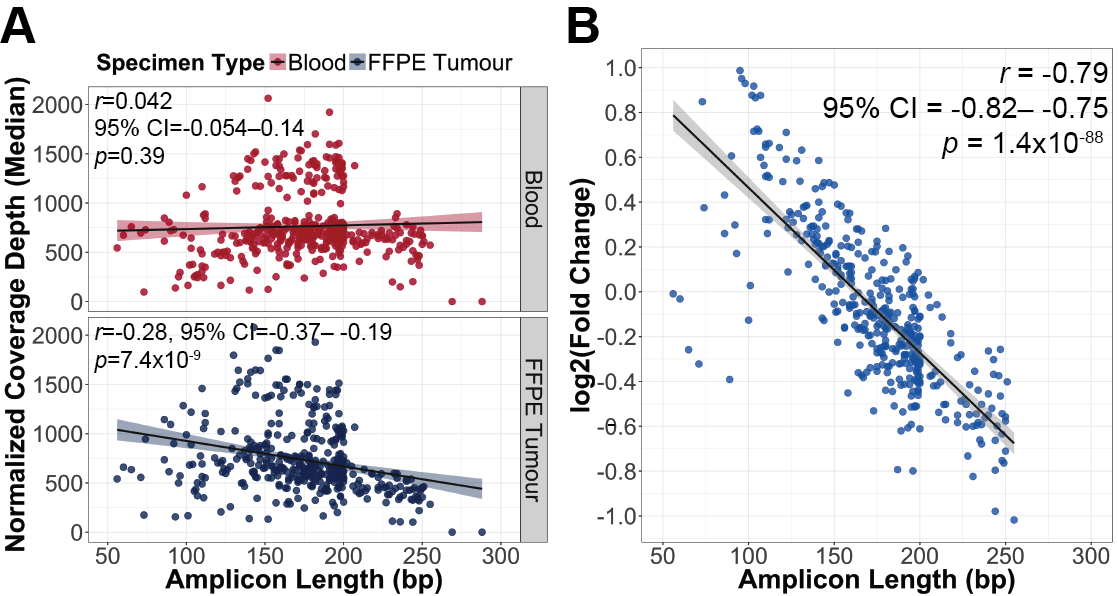
\includegraphics[scale=0.85]{amp_cov_lm_len.png}
	\caption{The effect of amplicon length on coverage depth of amplicons. Coverage depth of amplicons was normalized to account for difference in library size and log2 fold change between the median coverage depth in blood and FFPE specimens (log2\( \frac{\text{Median Coverage Depth in FFPE}}{\text{Median Coverage Depth in Blood}} \)) was calculated for each amplicon. (A) No significant correlation between coverage depth of amplicons and amplicon length was demonstrated in blood specimens, whereas coverage depth of amplicons is negatively correlated with amplicon length in FFPE specimens (Pearson's correlation, \textit{p} $<$ 0.05). (B) Increased in amplicon length leads to lower log2 fold change in amplicon coverage depth between blood and FFPE specimens (Pearson's correlation, \textit{p} $<$ 0.05).}
	\label{fig:amp_cov_lm_len}
\end{figure}

%%%%%%%%%%%%%%%%%%%%%%%%%%%%%%%%%%%%%%%%%%%%%%%%%%%%%%%%%%%%%%%%%%%%%
%%%%%%%%%%%%%%%%%%%%%%%%%%%%%%%%%%%%%%%%%%%%%%%%%%%%%%%%%%%%%%%%%%%%%

\begin{figure}[H]
	\centering
	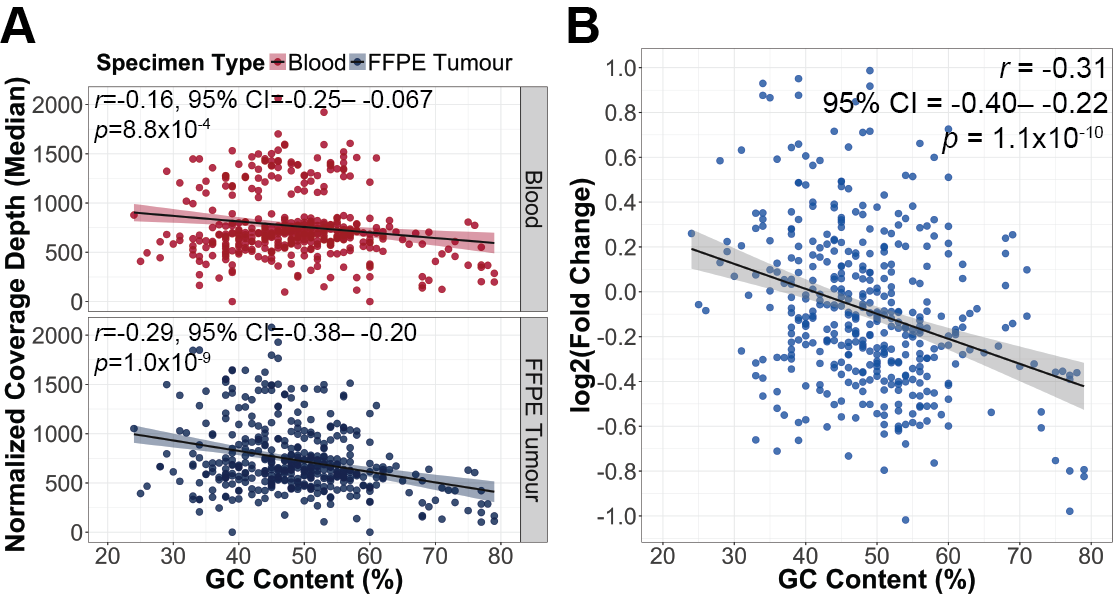
\includegraphics[scale=0.85]{amp_cov_lm_gc.png}
	\caption{The effect of amplicon GC content on coverage depth of amplicons. Coverage depth of amplicons was normalized to account for difference in library size and log2 fold change between the median coverage depth in blood and FFPE specimens (log2\( \frac{\text{Median Coverage Depth in FFPE}}{\text{Median Coverage Depth in Blood}} \)) was calculated for each amplicon. (A) Coverage depth of amplicons is negatively correlated with amplicon GC content in both blood and FFPE specimens (Pearson's correlation, \textit{p} $<$ 0.05). (B) Increased in amplicon GC content leads to lower log2 fold change in amplicon coverage depth between blood and FFPE specimens (Pearson's correlation, \textit{p} $<$ 0.05).}
	\label{fig:amp_cov_lm_gc}
\end{figure}
